% !TEX root = ../my-thesis.tex
%
\chapter{Calibration of catalytic efficiencies in reusable Thermal Protection Materials.}
\label{sec:cfd}

\cleanchapterquote{To call in the statistician after the experiment is done may be no more than asking him to perform a postmortem examination.}{Ronald Fisher}{(English Statistician, 1890-1962)}

\section{Introduction}
\label{sc:cfd:introduction}

This chapter illustrates a calibration problem in the field of hypersonic aerothermodynamics, which stems from a collaboration with the \gls{vki}. The primary interest of this collaboration was to explore the use of calibration techniques to reconstruct the catalytic efficiencies of reusable \glspl{tpm} from experimental measurements collected in the facilities of the \gls{vki}. The field of hypersonic aerothermodynamics is notoriously complex to approach, both from an experimental and a numerical perspective. The complexity of the physical phenomena involved, the high costs of the experimental campaigns, and the complexity of the numerical models used to simulate the experiments, make this field a perfect candidate for the application of \gls{uq} techniques. In particular, the calibration of the catalytic efficiencies of reusable \glspl{tpm} is a challenging problem, as it involves an interplay between potentially biased or incomplete experimental measurements and numerical models affected by model error.

\smallskip
The goal of this chapter is to introduce the problem from both an experimental and numerical perspective, illustrating the challenges involved in both aspects. In particular, after a brief introduction to the field and the relevant state-of-the-art in~\S\ref{sc:cfd:motivation}, we describe the Plasmatron facility at the \gls{vki}, detailing the quantities that can and cannot be measured in~\S\ref{sc:cfd:plasmatron}. Consequently, we also formulate the calibration problem. In \S\ref{sc:cfd:numericalmodel}, we describe the numerical models used to simulate the hypersonic jet, i.e. a high fidelity \gls{cfd} model and a low-fidelity model based on some simplifying assumptions. In the same section we also introduce the \gls{gsi} model used to simulate the interaction between the jet and the \gls{tpm} sample. Finally, in \S\ref{sc:cfd:methodology}, we derive the calibration framework used to reconstruct the catalytic efficiencies from the experimental measurements. In \S\ref{sc:cfd:results} we present the results of the calibration on a \textit{synthetic} demonstration campaign, as well as an application of the \gls{cmp} and \gls{as}-\gls{hgp} to this problem. Finally, in \S\ref{sc:cfd:conclusions} we summarize the main findings of this chapter and provide some concluding remarks.


\section{Motivation and State of the Art}
\label{sc:cfd:motivation}

During hypersonic re-entry, a spacecraft’s kinetic energy is transformed into thermal energy across the bow shock, generating a high-enthalpy flow that can heat the surface above $2000$\,K. \glspl{tpm} are therefore essential to preserve structural integrity and ensure mission safety. In relatively moderate re-entry conditions (e.g., Earth-entry velocities below $10$\,km/s), where peak heat fluxes can be tolerated without severe material recession, reusable catalytic \glspl{tpm} are typically employed \cite{vignoles2018ablative}. Under these conditions, a substantial portion of the incoming energy is re-radiated from the hot surface to the flow, while the remaining part is transferred by conduction into the \gls{tpm}. These materials are usually carbon- or silicon-carbide-based and are designed to combine high emissivity, which enhances radiative cooling, with low catalytic activity, which limits surface recombination reactions of atomic species \cite{laub2004thermal}.

\smallskip
Due to the complex multiphysics phenomena occurring between the shock layer and the \gls{tpm}, such as thermochemical non-equilibrium and \gls{gsi}, the design of reusable \glspl{tpm}, and especially the assessment of their catalytic efficiencies, remains challenging. In this context, \gls{gsi} denotes coupled mass and heat transfer at the surface, where strong velocity and temperature gradients drive reactive species toward the wall and promote heterogeneous reactions. From a modeling perspective, catalytic reactions are commonly represented through catalytic efficiencies. Because these efficiencies cannot be measured directly, they are typically inferred from experimental observables (e.g., stagnation heat flux) using inverse modeling approaches. Robust \gls{tpm} characterization therefore relies on combining advanced ground-based measurements (e.g., high-enthalpy wind tunnels) with numerical simulations~\cite{PhDThesis_Bellas}. Although such facilities reproduce flight-representative thermal loads under controlled conditions, extensive campaigns are costly and time-consuming, making computationally efficient physicochemical models essential. Since these models are mathematical representations of the underlying physics and inevitably include assumptions and simplifications, \gls{uq} methods are essential~\cite{PhDThesis_Capriati}.

\smallskip
In the hypersonic community, Upadhyay et al.~\cite{Upadhyay_2011} were the first to apply \gls{uq} methods to \gls{gsi} analysis. They adopted a Bayesian framework~\cite{kaipio2005,uq_theory} to estimate the nitrogen efficiency. Bayesian inference provided a rigorous framework to quantify uncertainty in model parameters by combining experimental observations with their associated uncertainties. Sanson et al.~\cite{SANSON2018482} reconstructed catalytic properties from measurements collected at the \gls{vki} Plasmatron facility \cite{Plasmatron, el2024upgraded}. They showed that Bayesian methods can infer \gls{tpm} catalytic properties even with a limited number of experiments. Further insights into \gls{gsi} in reusable \glspl{tpm} were provided by del Val et al.~\cite{DelVal_2022}, who introduced a Bayesian formulation that explicitly includes nuisance parameters, i.e., variables required for inference but not targeted for calibration. While effective, the approaches in~\cite{SANSON2018482} and~\cite{DelVal_2022} were limited to high-enthalpy subsonic flows. Capriati et al.~\cite{Capriati2024} extended this line of work to \gls{gsi} characterization in under-expanded high-enthalpy jets, typically used to obtain higher heat-flux levels, closer to effective values, on \gls{tpm} samples. In all these studies, the complex physical phenomena were represented through \gls{cfd} simulations.

\smallskip
A key limitation of previous studies is that the discrepancy between simulations and measurements was attributed only to experimental uncertainty. In high-enthalpy plasma facilities, this assumption is often overly optimistic. Del Val et al.~\cite{del2026modelerror} noted that ground-test facilities cannot reproduce the full range of physical phenomena and timescales encountered in flight. As a consequence, models calibrated on incomplete experimental datasets may exhibit significant predictive errors, because inferred parameters can absorb multiple un-modeled effects, reducing generalizability. For example, calibrating gas-phase chemical-kinetic mechanisms without accounting for these gaps can introduce uncertainties that propagate to predicted shock-layer composition and resulting boundary layer gradients. The role of model error in hypersonic applications was also emphasized by Capriati~\cite{PhDThesis_Capriati}. After calibrating a finite-rate air-carbon ablation model, he observed that predicted mass blowing rates were less sensitive to surface temperature than suggested by experiments. This mismatch may indicate model inadequacy, measurement bias, or both. Additional sources of model error include simplified \gls{gsi} treatments (e.g., prescribing a fixed catalytic efficiency instead of resolving finite-rate surface chemistry), diffusion-model assumptions, numerical errors (e.g., insufficient near-wall mesh resolution), and assumptions embedded in simulations (e.g., uniform reservoir conditions in high-enthalpy plasma wind-tunnel testing). Neglecting these effects can induce bias and promote overfitting in parameter estimation~\cite{hagan_2014, ling2014selection}.

\section{Calibration of Plasmatron data}
\label{sc:cfd:plasmatron}

This section briefly describes the experimental facility and the real supersonic campaign that the synthetic data used for the Bayesian inversion are intended to reproduce.

\subsection{The Plasmatron Facility}
The \gls{vki} Plasmatron is the most powerful inductively-coupled-plasma wind tunnel worldwide. It features a plasma torch driven by a high-frequency, high-power, high-voltage generator, allowing ground-based simulation of the high-enthalpy flow and chemically reacting boundary layers developing over a re-entry vehicle. The Plasmatron facility can maintain high-enthalpy conditions for long durations, making it especially suitable for \gls{tpm} characterization. 

\smallskip
In the Plasmatron, a high-purity plasma is produced by inductively heating a gas inside a coil and expanding it as a jet into a sub-atmospheric test chamber, with no direct contact between the plasma and the facility components. This contact-free configuration reduces plasma contamination, which would otherwise increase \gls{tpm} catalytic activity. Additional details on the facility are provided in~\cite{Plasmatron}.

\smallskip
The experimental setup used by El Rassi et al.~\cite{el2024upgraded} is schematically shown in Fig.~\ref{fig:Expsetup}. The plasma flow is generated in the torch (a), expanded through a convergent-divergent nozzle (b), and then discharged into the test chamber (c). A calorimeter (d), with a radius of 25\,mm and located 42.9\,mm downstream of the nozzle, was used to monitor the stagnation-point heat flux $q_\mathrm{w}$. A snapshot of the real supersonic jet is reported in Fig.~\ref{fig:SupJet}.

\begin{figure}[htbp]
    \centering
    \begin{subfigure}[t]{0.47\textwidth}
        \centering
        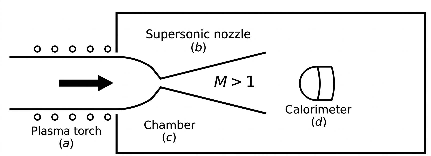
\includegraphics[width=\textwidth]{figures/cfd/ExpSetUp_v2.pdf}
        \caption{\gls{vki} Plasmatron experimental set-up.}
        \label{fig:Expsetup}
    \end{subfigure}
    \quad
    \begin{subfigure}[t]{0.45\textwidth}
        \centering
        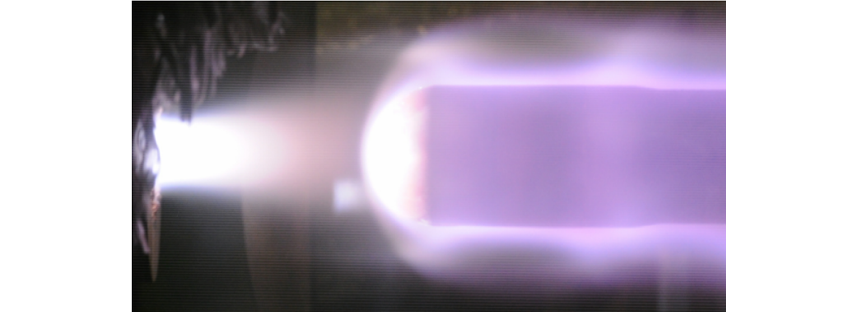
\includegraphics[width=\textwidth]{figures/cfd/SupersonicJet.pdf}
        \caption{Supersonic under-expanded air jet (credit:~\cite{Capriati2024}).}
        \label{fig:SupJet}
    \end{subfigure}

    \caption{The supersonic campaign at the \gls{vki} Plasmatron facility. On the left, the experimental set-up is shown. On the right, a snapshot of the supersonic jet is reported.}
    \label{fig:SupersonicExpCamp}
\end{figure}

The control variables of the facility are the power supplied to the torch $Q_{\text{torch}}$, the chamber static pressure $\mathrm{P}_{\text{s}}$, and the mass flow rate $\dot{m}$. The latter is regulated by a mass flow controller, while absolute pressure sensors measure the reservoir pressure $\mathrm{P}_{0}$. The accuracy of each pressure sensor is 1\%, and the accuracy of the mass flow controller is 0.5\%. A measurement probe is positioned at the stagnation point of the jet to measure the stagnation heat-flux (with a calorimeter) $q_\mathrm{w}$, and the stagnation pressure $\mathrm{P}_\mathrm{w}$ (with a pressure sensor). The accuracy of the heat-flux measurement is estimated to be around 5\%, while the accuracy of the pressure sensor is 1\%. The probe is water-cooled and maintained at approximately 350\,K. Control variables and measured quantities are summarized in Tab.~\ref{tab:SupersonicCampaign} along with the corresponding uncertainty.

\begin{table}[htbp]
\centering
\caption{Control variables and measured quantities for the supersonic \gls{vki} Plasmatron campaign together with the corresponding uncertainty.}
\begin{tabular}{cc|cc}
\hline
Control variables & Uncertainty & Measured quantities & Uncertainty\\
\hline
Torch power, $Q_{\text{torch}}$ & -- & Stagnation heat-flux, $q_\mathrm{w}$ & $\pm 5\%$ \\
Mass flow rate, $\dot{m}$ & $\pm 0.5\%$ & Reservoir pressure, $\mathrm{P}_0$ & $\pm 1\%$ \\
Chamber static pressure, $\mathrm{P}_\text{s}$ & $\pm 1\%$ & Stagnation pressure, $\mathrm{P}_\mathrm{w}$ & $\pm 1\%$ \\
\hline
\end{tabular}
\label{tab:SupersonicCampaign}
\end{table}

It is important to note that, at the current stage, the total temperature $\mathrm{T}_0$ cannot be directly measured in the facility. For these reasons, it is important to infer it from the available measurements, which is one of the goals of the calibration process. The same applies to the catalytic efficiencies of the probe, which are also inferred from the available measurements. In the next section, we present the \gls{cfd} model used to simulate the experiment and generate synthetic data for the calibration process.

\subsection{Definition of the Calibration Problem}

To reconstruct the catalytic efficiencies, we need to identify a suitable set of observables that are sensitive to the parameters of interest. Given the experimental setup described in the previous section, we choose to use the stagnation heat-flux $q_\mathrm{w}$, as it is the only observable that is sensitive to the catalytic efficiencies. The stagnation pressure $\mathrm{P}_\mathrm{w}$ and the mass flow rate $\dot{m}$, instead, are not sensitive to the catalytic efficiencies, as they are determined by the flow conditions in the reservoir and the chamber, which are not affected by the \gls{gsi} phenomena occurring at the probe surface. The total temperature $\mathrm{T}_0$ cannot be used as an observable, as it is not directly measured in the facility. 
The calibration problem can be mathematically formulated as follows:

\begin{equation}
  q_\mathrm{w} = \tilde{q}_\mathrm{w}(\mathbf{x}; \boldsymbol{\gamma}) + z_{q_\mathrm{w}}(\mathbf{x}) + \epsilon_{q_\mathrm{w}}(\mathbf{x}) \quad \text{with} \quad \mathbf{x} = (\mathrm{P}_0, \mathrm{P}_s, \dot{m}) \;.
  \label{eq:cfd:cali_1}
\end{equation}

In Eq.~\eqref{eq:cfd:cali_1}, $\tilde{q}_\mathrm{w}$ is the prediction of the computer code, which depends on the control variables $\mathbf{x}$ and the parameters of interest $\boldsymbol{\gamma} = (\gamma_N, \gamma_O)$. The term $z_{q_\mathrm{w}}$ is the model error term, which accounts for the discrepancy between the computer code and the real experiment. Finally, $\epsilon_{q_\mathrm{w}}$ is the measurement error term, which accounts for the uncertainty in the measurements. The latter is assumed to be Gaussian with zero mean and a standard deviation of 5\% of the measured value, as reported in Tab.~\ref{tab:SupersonicCampaign}. 

\smallskip
A second possibility, would be to treat the total temperature $\mathrm{T}_0$ as a nuisance parameter, and to include it in the calibration process. In this case, the calibration problem can be mathematically formulated as follows:

\begin{equation}
  \left.
  \begin{aligned}
    &q_\mathrm{w} = \tilde{q}_\mathrm{w}(\mathbf{p}; \gamma_{\mathrm{N}}, \mathrm{T}_0) + z_{q_\mathrm{w}}(\mathbf{p}) + \epsilon_{q_\mathrm{w}}(\mathbf{p}) \\
    &\mathrm{P}_\mathrm{w} = \hat{\mathrm{P}}_\mathrm{w}(\mathbf{p}; \gamma_{\mathrm{N}}, \mathrm{T}_0) + z_{\mathrm{P}_\mathrm{w}}(\mathbf{p}) + \epsilon_{\mathrm{P}_\mathrm{w}}(\mathbf{p}) \\
    &\dot{m} = \hat{m}(\mathbf{p}; \gamma_{\mathrm{N}}, \mathrm{T}_0) + z_{\dot{m}}(\mathbf{p}) + \epsilon_{\dot{m}}(\mathbf{p}) \;,
  \end{aligned}
  \right.
  \label{eq:cfd:cali_2}
\end{equation}

with $\mathbf{p} = (\mathrm{P}_0, \mathrm{P}_s)$ the pressure variables. In this case, the calibration problem is more complex, as we need 3 observables and 3 model error terms. Notice that we do not calibrate $\gamma_O$ in this case, for simplicity. Eq.~\eqref{eq:cfd:cali_2} is the formulation of the calibration problem that we will use in the second part of this chapter, where we apply the \gls{cmp} framework to reduce the dimensionality of the calibration problem and make it tractable.  

\smallskip
At this stage, the calibration problem is well-defined, and we proceed in \S\ref{sc:cfd:numericalmodel} with a description of the different numerical models used in the results, which are presented in \S\ref{sc:cfd:results}. \S\ref{sc:cfd:methodology} gives additional details on the methodology used to build the surrogate models of the numerical codes and how training and synthetic data are generated for the calibration process.


\section{Numerical Models}
\label{sc:cfd:numericalmodel}

In this section, we present two numerical models used to simulate the experiment. The first one is a high-fidelity \gls{cfd} model that solves the multi-component \gls{ns} equations for a mixture of chemically reacting species in thermochemical non-equilibrium. The second one couples a 0D nozzle solver with a quasi-1D solver that reproduces the flow field along the stagnation line of the probe. 

\subsection{High fidelity solver}
\label{sc:cfd:us3D}

The \gls{cfd} solver \texttt{US3D} (version 1.1.8)~\cite{US3D} is a parallel, implicit, unstructured, three-dimensional flow solver developed at the University of Minnesota in collaboration with NASA for the accurate simulation of hypersonic and re-entry flows. The high-temperatures and relatively low-pressures that characterize the applications considered in this work activate chemical reactions that alter the gas composition and promote dissociation. \texttt{US3D} is used to solve the multi-component \gls{ns} equations for a mixture of \(n_\text{s}\) chemically reacting species in thermochemical non-equilibrium:


\begin{equation}
  \left\{
\begin{aligned}
  &\frac{\partial \rho_i}{\partial t} + \nabla \cdot (\rho_i \mathbf{u} + \mathbf{j}_i) = \dot{\omega}_i, \quad \forall i \in [1, n_{\text{s}}]\\
  &\frac{\partial (\rho \mathbf{u})}{\partial t} + \nabla \cdot \left(\rho \mathbf{u} \otimes \mathbf{u} + \mathrm{P} \mathbf{I} + \mathbf{T}\right) = \mathbf{0} \\
  &\frac{\partial (\rho e)}{\partial t} + \nabla \cdot \left(\rho\mathbf{u} h + \mathbf{T} \cdot \mathbf{u} + \mathbf{q}\right) = 0.
\end{aligned}
\label{eq:cfd:ns}
\right.
\end{equation}

In Eq.~\ref{eq:cfd:ns}, $\rho_i$ stands for the partial density of species $i$, $\mathbf{u}$ is the mass-averaged velocity of the mixture, $\mathbf{j}_i$ the diffusion mass flux of species $i$, and $\dot{\omega}_i$ its chemical production/destruction rate. The terms $\rho$ and $\mathrm{P}$ are, respectively, the density and the thermodynamic pressure of the mixture, $\mathbf{T}$ refers to the viscous stress tensor, while, $e$ stands for the specific internal energy, and $h$ is the total enthalpy. Neglecting radiative contributions, $\mathbf{q}$ is the total heat flux, including both conductive and diffusive components. 

\smallskip
The thermodynamic properties of the mixture necessary to close the \gls{ns} system are computed using the \texttt{MUTATION++} library~\cite{polynomialNASA, MUTATIONPP, capriati2021development}. Species diffusion fluxes are calculated using self-consistent effective binary diffusion models \cite{Ramshaw}, while the viscosity and thermal conductivity are evaluated following the method of Gupta et al.~\cite{ViscosityThermalCond}.

\smallskip
Furthermore, we consider the finite-rate chemistry of a 5-species air mixture (\(\text{N}_2, \text{O}_2, \text{NO}, \text{N}, \text{O}\)) assuming laminar, steady, and in thermal equilibrium flow, with rate coefficients taken from Park et al.~\cite{Park}. The modified Steger–Warming flux vector splitting scheme~\cite{StegerWarming} is used to compute convective fluxes in steady-state simulations, combined with a MUSCL reconstruction~\cite{MUSCL} to achieve second-order accuracy. Spatial discretization is based on the finite volume method, and rapid convergence to steady state is obtained using the full-matrix point relaxation approach~\cite{FMPR}.

\begin{figure}[htbp]
    \centering
    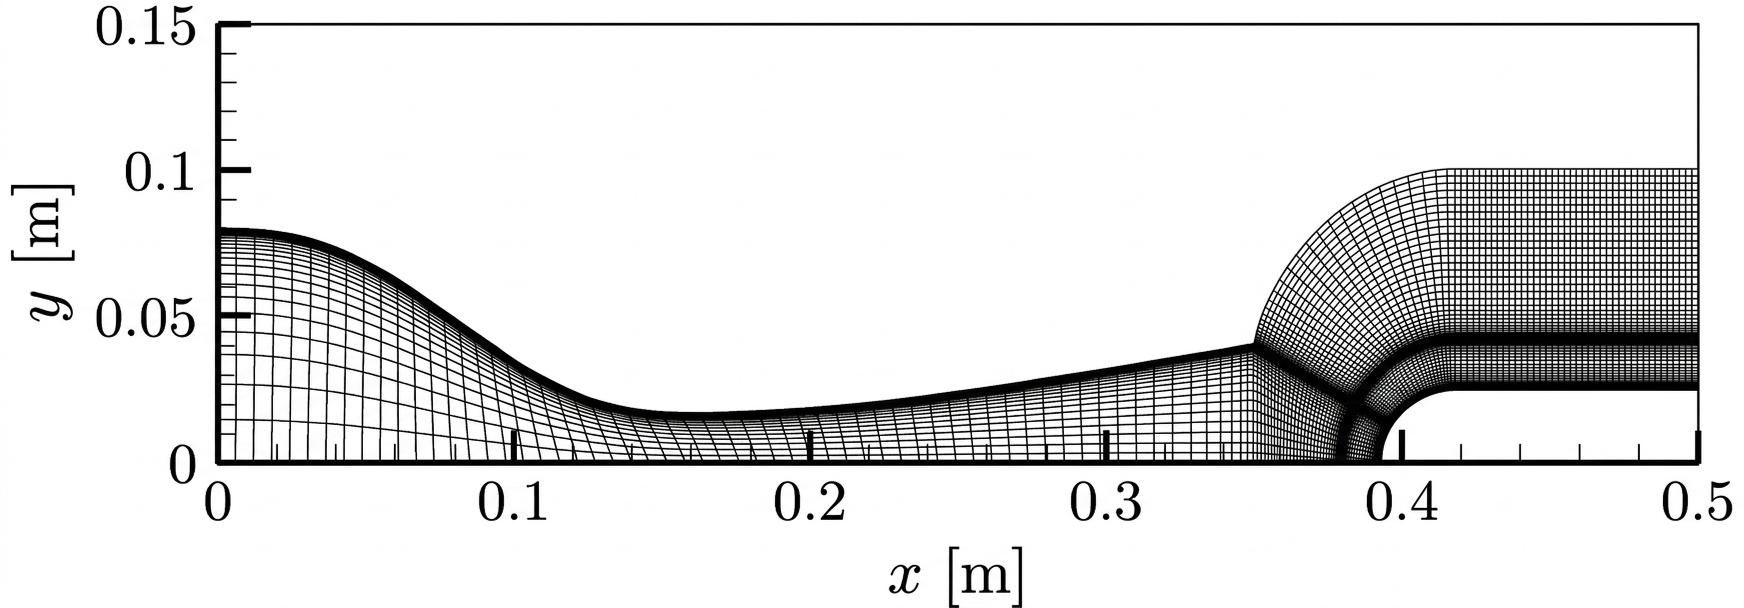
\includegraphics[width=0.8\textwidth]{figures/cfd/MeshTecplot.pdf}
    \caption{Numerical domain and mesh used for the \gls{cfd} simulations.}
    \label{fig:NumericalDomain}
\end{figure}

The numerical domain corresponds to the region between the nozzle inlet (i.e. the exit of the torch) and the stagnation point of the probe. Since a bow shock develops in front of the probe, the mesh is aligned with the shock to ensure accurate resolution of the flow field and reliable stagnation heat-flux values.

As far as the boundary conditions are concerned, a subsonic inflow condition is prescribed at the nozzle inlet. Accordingly, the reservoir pressure $\mathrm{P}_0$ and temperature $\mathrm{T}_0$, together with the inflow velocity $\mathbf{u}_0$. The chemical composition of the inflow is defined by imposing chemical equilibrium at the reservoir conditions. The nozzle walls are modeled as isothermal, non-catalytic surfaces with a fixed temperature of \(350\,\text{K}\). A supersonic outflow condition is imposed at the outlet section. The probe is modeled as an isothermal, catalytic surface with a fixed temperature of \(350\,\text{K}\). All other boundaries are treated as symmetry planes. 


\subsection{Low fidelity solver}

In this section, we present a low-fidelity solver that we use as a way to synthetically introduce a model error term in the calibration process. The low fidelity solver is built by coupling a simple 0D nozzle solver with a quasi 1D solver that reproduces the flow field along the stagnation line of the probe. 

\begin{figure}[htbp]
    \centering
    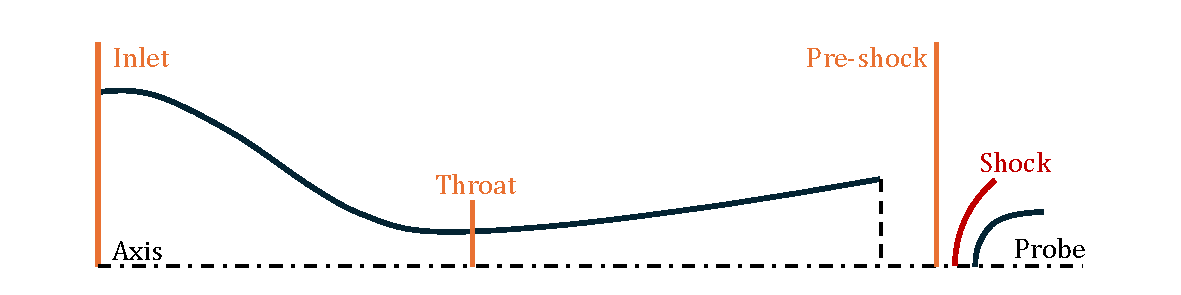
\includegraphics[width=0.8\textwidth]{figures/cfd/LowFidelity.pdf}
    \caption{Sketch of an under-expanded jet over a probe.}
    \label{fig:LowFidelity}
\end{figure}

Fig.~\ref{fig:LowFidelity} shows a sketch of the domain considered for the low-fidelity solver. The reservoir pressure $\mathrm{P}_0$ and temperature $\mathrm{T}_0$, are given as input conditions to a 0D nozzle solver that returns the gas state at different positions in the nozzle. The solver imposes the conservation of total pressure and total enthalpy, full chemical equilibrium at the inlet, sonic conditions at the throat, and frozen chemistry along the stagnation line. Note that the position of the shock and the jet diameter are not fixed, but depend on the reservoir and chamber conditions. To overcome this issue, we model these quantities by interpolating three high fidelity \gls{cfd} simulations. The gas state in the pre-shock region is then fed to the \texttt{STAGLINE} solver~\cite{STAGLINE}, which is used to compute the flow field along the stagnation line of the probe. \texttt{STAGLINE} is a quasi-1D material-response \gls{cfd} solver that reproduces the flow-field along the stagnation line of a spherical body under the assumptions of steady, laminar, axi-symmetric flow. The dimensionality of the problem is reduced by adopting the dimensionally reduced \gls{ns} equations formulation~\cite{DRNSE}. The spatial discretization of the conservation equations relies on a finite volume method, while an implicit backward-Euler scheme is used for time integration. Numerical fluxes are computed with the Roe scheme~\cite{ROEscheme} and transport properties, instead, from the kinetic theory of gases using a Chapman-Enskog perturbative solution method to the Boltzmann equation~\cite{MAGIN_Transport_Properties}. \texttt{STAGLINE} has also been coupled with the \texttt{MUTATION++} library~\cite{MUTATIONPP}, which is used to compute the chemical production rates and the thermodynamic properties of the mixture.

\subsection{Gas-Surface Interaction: Gamma Model}
\label{subsubsec:GSI}

Finally, in this last subsection, we give more insights into the modeling of the \gls{gsi} phenomena, which is the key modeling aspect of this test case. 
The \gls{gsi} phenomena are driven by the recombination of atomic species at the surface, which can be represented by the following reactions:

\begin{equation}
    \text{N} + \text{N} \rightarrow \text{N}_2 \quad \text{and} \quad \text{O} + \text{O} \rightarrow \text{O}_2.
\end{equation}

Since these recombination reactions are exothermic, they increase the heat-flux that directly affects \gls{tpm} design. Since we are dealing with a purely catalytic surface, the resulting surface-mass-balance for each species $i$ states that the catalytic activity is equivalent to the diffusion flux to the surface: 

\begin{equation}
    \textbf{j}_i \cdot \hat{\textbf{n}} = \dot{\Omega}_{\text{cat},i} \quad \forall i \in [1, n_{\text{s}}],
    \label{eq:SMB}
\end{equation}

where $\textbf{j}_i$ is the diffusion mass flux, $\textbf{n}$ is the normal to the surface, and ˙$\dot{\Omega}_{\text{cat},i}$ is the surface source term only due to catalytic chemical reactions. 

To close the SMB equations, we need to specify the chemical production rates $\dot{\Omega}_{\text{cat}}$. In this work, we choose to adopt a phenomenological approach, which is the most common in the hypersonic community, called the \textit{Gamma Model}~\cite{GammaModel}. Note that different approaches exist in the literature, such as finite-rate chemistry models~\cite{FRC}. The approach behind the Gamma Model is to introduce a catalytic efficiency $\gamma_i$ for each species $i$, which represents the probability that a macroscopic reaction occurs when a molecule of species $i$ impinges on the surface. This probability can be interpreted as the ratio between the number of molecules of species $i$ that react at the surface $N_i^{\star}$ and the number of molecules of species $i$ that impinge on the surface $N_i$, i.e.,


\begin{equation}
    \gamma_i=\dfrac{N_i^{\star}}{N_i},
\end{equation}

The total number of impinging molecules of species $i$ is computed through the Boltzmann distribution, as $N_i=(\rho_i/m_i)\sqrt{(\mathrm{k}_{\text{b}}\mathrm{T}_\text{s})/(2\pi m_i)}$. The symbol $\mathrm{k}_{\text{b}}$ represents Boltzmann's constant, $\mathrm{T}_{\text{s}}$ denotes the surface temperature, and $m_i$ refers to the mass of species $i$. When the probability approaches unity, the surface is said to be fully catalytic. Conversely, when the probability is equal to zero, the surface is said to be non-catalytic. The concept of partial catalysis falls within the range defined by these two limits. Finally, the chemical production reads: 

\begin{equation}
    \dot{\Omega}_{\text{cat},i} = m_i \gamma_i N_i.
\label{eq:omega}
\end{equation} 

\section{Methodology}
\label{sc:cfd:methodology}

We are now going to describe the methodology used to perform the calibration of the computer code. First and foremost, we set the true values of the efficiencies to $\gamma_N = 0.0736$ and $\gamma_O = 0.1170$, which are taken from the work of~\cite{PhDThesis_Bellas}. Secondly, we need to address the differences between the mapping of the computer code and the mapping of the experiment. Indeed, both \texttt{STAGLINE} and \texttt{US3D} are structured with the following mapping


\begin{equation}
    \left.
    \begin{aligned}
        &\text{Control variables} \times \text{Parameters} \rightarrow \text{Observables} \\
        &\left( \text{P}_0, \text{P}_s, \mathrm{T}_0\right) \times (\gamma_N, \gamma_O) \rightarrow \left( q_{\mathrm{w}}, \text{P}_w, \dot{m}\right) \;.
    \end{aligned}
    \right.
    \label{eq:cfd:mapping}
\end{equation}

The main issue behind Eq.~\eqref{eq:cfd:mapping} is that experimentalists do not have access to measurements of the total temperature $\mathrm{T}_0$, which is a key input for the \gls{cfd} solver. To circumvent this issue, we first build a surrogate model of the two computer codes using a training dataset over the following bounds:

\begin{table}[htbp]
  \centering
  \caption{Training bounds used to build the surrogate model.}
  \label{tab:cfd:training_bounds}
  \begin{tabular}{lccccc}
    \toprule
    Bound type & $\text{P}_0$ [kPa] & $\text{P}_s$ [Pa] & $\mathrm{T}_0$ [K] & $\log_{10}\gamma_N$ [-] & $\log_{10}\gamma_O$ [-] \\
    \midrule
    low & 11.5 & 200 & 4000 & -4 & -4 \\
    up  & 21.5 & 400 & 7000 & 0 & 0 \\
    \bottomrule
  \end{tabular}
\end{table}

A total of 160 \gls{cfd} simulations (using \texttt{US3D}) and 300 simulations (using \texttt{STAGLINE}) are performed to build the surrogate model. The training dataset is built using a \gls{lhs} strategy, a space-filling design that ensures a good coverage of the input space.

\begin{figure}[htbp]
    \centering
    \begin{subfigure}[t]{0.47\textwidth}
        \centering
        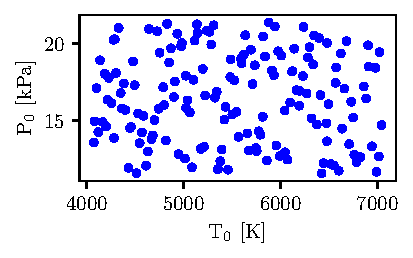
\includegraphics[width=\textwidth]{figures/cfd/bounds_plot.pdf}
        \caption{Numerical \gls{doe} for \texttt{US3D} projected in the $\mathrm{T}_0$ vs $\mathrm{P}_0$ coordinates.}
        \label{fig:TrainingDataUS3D}
    \end{subfigure}
    \quad
    \begin{subfigure}[t]{0.47\textwidth}
        \centering
        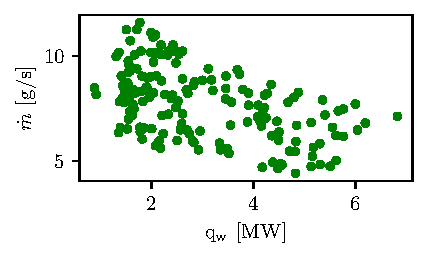
\includegraphics[width=\textwidth]{figures/cfd/bounds_plot_Qw_Mdot.pdf}
        \caption{Image of the \gls{doe} via \texttt{US3D} projected in the $q_{\mathrm{w}}$ vs $\dot{m}$ coordinates.}
        \label{fig:TrainingDataSTAGLINE}
    \end{subfigure}

    \caption{Training dataset constructed using \texttt{US3D} simulations.}
    \label{fig:cfd:DoE}
\end{figure}

The numerical \gls{doe} constructed using \texttt{US3D} is shown in Fig.~\ref{fig:cfd:DoE}, projected in the $\mathrm{T}_0$-$\mathrm{P}_0$ (input) and $q_{\mathrm{w}}$-$\dot{m}$ (output) coordinates. As we can see from Fig.~\ref{fig:TrainingDataSTAGLINE}, the image of the \gls{doe} via the computer code shows a good coverage of the co-domain. 

\smallskip
A multi-output constant mean and a Matérn-52 elliptic covariance function \gls{gp} is used to build a surrogate model of the computer code using the previously described training dataset. To deal with the multi-output nature of the mapping, we use the same technique described in \S\ref{sc:surr:surrogate} that consists in scaling the y-coordinates using a \gls{pca} and then feeding the de-correlated outputs to a series of independent \glspl{gp}. When building the surrogate model, we perform a change of coordinates to be consistent with the calibration problem defined in Eq.~\eqref{eq:cfd:cali_1}. In particular, we swap the columns corresponding to $\mathrm{T}_0$ and $\dot{m}$, so that the mapping of the surrogate model becomes:

\begin{equation}
    \left.
    \begin{aligned}
        &\text{Control variables} \times \text{Parameters} \rightarrow \text{Observables} \\
        &\left( \text{P}_0, \text{P}_s, \dot{m}\right) \times (\gamma_N, \gamma_O) \rightarrow \left( q_{\mathrm{w}}, \text{P}_w, \mathrm{T}_0\right) \;.
    \end{aligned}
    \right.
    \label{eq:cfd:mapping_2}
\end{equation}

Eq.~\eqref{eq:cfd:mapping_2} is consistent with the calibration problem defined in Eq.~\eqref{eq:cfd:cali_1}, where $\dot{m}$ is treated as an observable and $\mathrm{T}_0$ as an output of the surrogate model. We will use only the heat-flux output of the surrogate model for calibration. The total temperature and wall pressure outputs, while not used for calibration, are useful for experimentalists (to discover the true value of the total temperature) and for predicting the wall pressure.

\begin{figure}[htbp]
    \centering
    \begin{subfigure}{0.47\textwidth}
        \centering
        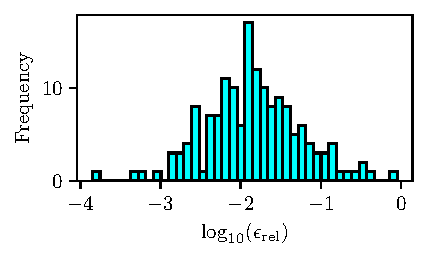
\includegraphics[width=\textwidth]{figures/cfd/loo_hist_us3d.pdf}
        \caption{\gls{loo}-\gls{cv} for the \texttt{US3D} surrogate.}
        \label{fig:loo_us3d}
    \end{subfigure}
    \quad
    \begin{subfigure}{0.47\textwidth}
        \centering
        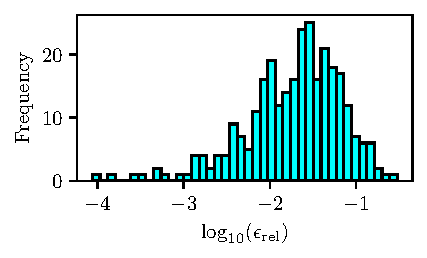
\includegraphics[width=\textwidth]{figures/cfd/loo_hist_stg.pdf}
        \caption{\gls{loo}-\gls{cv} for the STAGLINE surrogate.}
        \label{fig:loo_stg}
    \end{subfigure}
    \caption{\gls{loo}-\gls{cv} error of the heat-flux for the \texttt{US3D} and STAGLINE surrogates.}
    \label{fig:cfd:loo}
\end{figure}

The performance of the surrogate model is assessed through a \gls{loo}-\gls{cv} procedure. The results are shown in Fig.~\ref{fig:cfd:loo}, where the histograms of the relative \gls{loo} absolute errors for $\mathrm{q}_w$ are reported for both the \texttt{US3D} and \texttt{STAGLINE} surrogates. The relative \gls{loo} absolute error is defined as,

\begin{equation}
    \epsilon_{\mathrm{rel}, i} = \frac{|\tilde{q}_{-i}(\mathbf{x}_i) - y_i|}{|y_i|},
\end{equation}

where $\tilde{q}_{-i}(\mathbf{x}_i) = \mathbb{E}[\tilde{q}(\mathbf{x}_i) | \mathcal{D}_{-i}]$ is the \gls{loo} prediction for the $i$-th data point, and $y_i$ is the true value of the heat-flux for the $i$-th data point. As we can see from Fig.~\ref{fig:cfd:loo}, the surrogate model shows a good performance, with a mean relative error around $1\%$ for both surrogates. Regardless, any remaining model error is automatically accounted for in the calibration process through the model error term $z_{q_\mathrm{w}}$. 

\begin{table}[htbp] 
  \small
  \centering
  \begin{tabular}{|p{0.5cm}|p{1.5cm}|p{1.5cm}|p{1.5cm}|p{1.5cm}|p{2.2cm}| p{2.2cm}|} 
    \hline
    & \multicolumn{3}{|c|}{\textbf{Control variables}} &\multicolumn{3}{|c|}{\textbf{Observables}} \\ \cline{2-7} 
    & $P_0$ [kPa] & $P_s$ [Pa] & $\dot{m}$ [g/s] & $\mathrm{P}_{\mathrm{w}}$ [kPa] & $q_{\mathrm{w}}$ [MW/m$^2$] & T$_0$ [K] \\ \hline
      1 & 19.699 & 260 & 10.18 & 4.29962 & 1.9473 & 4777.59\\
      2 & 18.658 & 327 & 7.63 & 4.08939 & 3.86266 & 6409.65\\
      3 & 17.838 & 241 & 8.89 & 3.94114 & 2.16035 & 5054.2\\
      4 & 20.559 & 272 & 8.09 & 4.44787 & 4.7459 & 6552.7\\
      5 & 18.929 & 260 & 9.98 & 4.14516 & 1.83382 & 4651.85\\
      6 & 17.694 & 328 & 9.75 & 3.85677 & 1.53468 & 4377.64\\
      7 & 20.164 & 283 & 7.78 & 4.38786 & 4.9942 & 6719.74\\
      8 & 20.254 & 317 & 11.26 & 4.39298 & 1.83409 & 4196.9\\
      9 & 16.488 & 220 & 7.96 & 3.73369 & 2.41995 & 5327.5\\
      10 & 20.55 & 225 & 9.39 & 4.50978 & 2.73942 & 5544.63\\
      11 & 17.194 & 238 & 8.97 & 3.79204 & 1.91788 & 4773.95\\
      12 & 19.355 & 289 & 7.47 & 4.26912 & 4.9068 & 6719.05\\
    \hline
  \end{tabular}
  \caption{Synthetic data generated with the \gls{cfd} code using $\gamma_N = 0.0736$ and $\gamma_O = 0.1170$. }
  \label{tab:exp_data}
\end{table}

In Tab.~\ref{tab:exp_data}, we report the synthetic data generated with the \gls{cfd} code using $\gamma_N = 0.0736$ and $\gamma_O = 0.1170$. A total of 12 synthetic observations are generated from the \gls{cfd} code. To verify that the calibration problem is well-posed, i.e. that the heat flux $q_{\mathrm{w}}$ is sensitive enough to the catalytic coefficients $\gamma_N$ and $\gamma_O$, and that the newly defined mapping in Eq.~\eqref{eq:cfd:mapping_2} is bijective, we perform a global sensitivity analysis and a calibration with synthetic data generated from the surrogate model itself. The results of these analyses are reported in the next section.


\begin{figure}[htbp]
   \centering
    \begin{subfigure}[t]{0.47\textwidth}
        \centering
        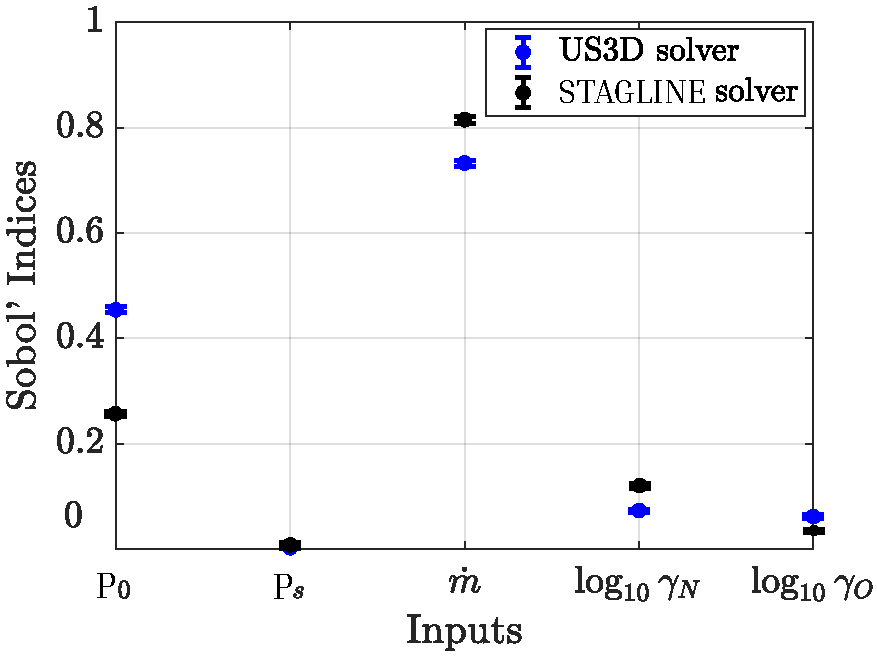
\includegraphics[width=\textwidth]{figures/cfd/Sensitivity_qw.pdf}
        \caption{Sobol' sensitivity indices for the heat-flux $q_{\mathrm{w}}$ (total indices).}
        \label{fig:cfd:sobol}
    \end{subfigure}
    \quad
    \begin{subfigure}[t]{0.47\textwidth}
        \centering
        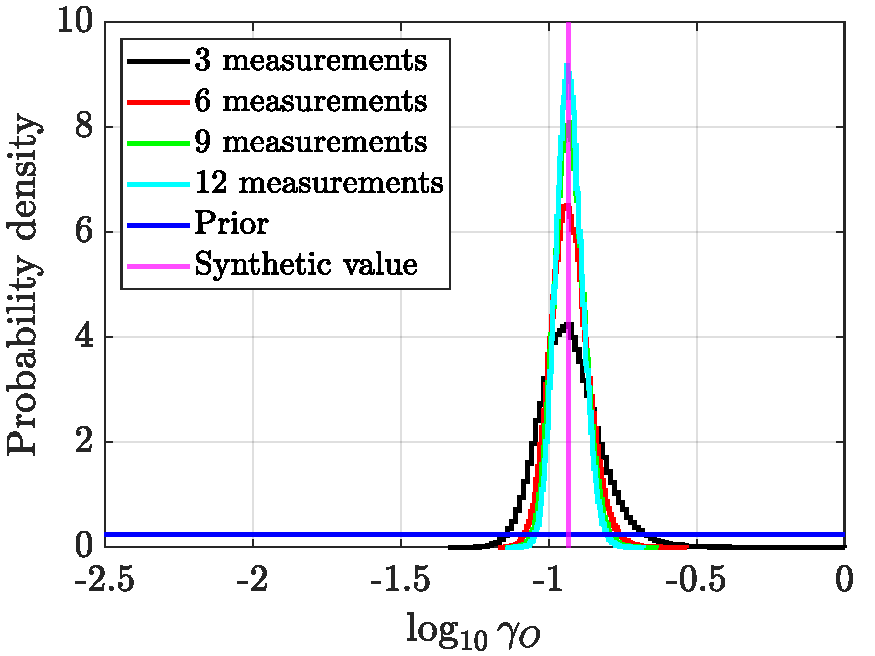
\includegraphics[width=\textwidth]{figures/cfd/Bayesian_gammaO.pdf}
        \caption{Posterior distribution of $\gamma_O$ obtained by calibrating the surrogate model with synthetic data generated from the surrogate model itself.}
        \label{fig:cfd:cali}
    \end{subfigure}
    \caption{Practical demonstration of the well-posedness of the calibration problem. On the left, the Sobol' sensitivity indices for the heat-flux $q_{\mathrm{w}}$ are reported. On the right, the posterior distribution of $\gamma_O$ obtained by calibrating the surrogate model with synthetic data generated from the surrogate model itself is shown.}
    \label{fig:cfd:wellpose}
\end{figure}

In Fig.~\ref{fig:cfd:wellpose} we report the results of the sensitivity analysis and of the calibration with synthetic data generated from the surrogate model itself. The sensitivity analysis, reported in Fig.~\ref{fig:cfd:sobol}, is performed using the Sobol' method, which is a variance-based global sensitivity analysis technique~\cite{uq_theory} that decomposes the variance of the model output into contributions from each input variable and their interactions. The results of the sensitivity analysis and the calibration show promising results, indicating that the problem is well-posed, and that measurements are informative enough to infer the true values of the catalytic coefficients (the posterior distribution of $\gamma_O$ is well concentrated around the true value, represented by the vertical line).

\bigskip
As far as the solution of the more complex calibration problem defined in Eq.~\eqref{eq:cfd:cali_2} is concerned, we perform a similar procedure to define the mapping of the surrogate model, which becomes:

\begin{equation}
    \left.
    \begin{aligned}
        &\text{Control variables} \times \text{Parameters} \rightarrow \text{Observables} \\
        &\left( \text{P}_0, \text{P}_s\right) \times (\gamma_N, \mathrm{T}_0) \rightarrow \left( q_{\mathrm{w}}, \text{P}_w, \dot{m}\right) \;.
    \end{aligned}
    \right.
    \label{eq:cfd:mapping_surr}
\end{equation}

In Eq.~\eqref{eq:cfd:mapping_surr} the total temperature $\mathrm{T}_0$ is now treated as a parameter to be inferred from the available measurements (fixing the oxygen catalytic coefficient $\gamma_O$ to its true value to maintain identifiability), while the mass flow rate $\dot{m}$ is treated as an observable. The resulting calibration problem corresponds to situations in which the total temperature $\mathrm{T}_0$ is not directly measurable, but fixed to some unknown reservoir condition and needs to be inferred from the available measurements. Having access to multiple \glspl{qoi} is beneficial for the calibration process, since the corresponding model needs to explain multiple measurements at the same time, which is more difficult and can lead to a more informative posterior distribution. This is well reflected in the form of the likelihood function, which is a product of three terms, one per each observable. Calling $\mathbf{z}(.) = (z_{q_{\mathrm{w}}}(.), z_{\mathrm{P}_{\mathrm{w}}}(.), z_{\dot{m}(.)})$ the model error terms associated with each observable, $\data = \{\data_{q_{\mathrm{w}}}, \data_{\mathrm{P}_{\mathrm{w}}}, \data_{\dot{m}}\}$ the set of the different measurements, the posterior distribution of the parameters $\btheta = (\mathrm{T}_0, \gamma_N)$ can be written as follows:

\begin{equation}
  \p{\btheta, \boldsymbol{\psi} \mid \data} \propto \prior{\btheta} \prod_{i \in \{q_{\mathrm{w}}, \mathrm{P}_{\mathrm{w}}, \dot{m}\}} \prior{\bpsi_i} \, \p{\data_i \mid \btheta, \bpsi_i} \;.
  \label{eq:cfd:multi_post}
\end{equation}

Eq.~\eqref{eq:cfd:multi_post} reports the posterior distribution of the parameters $\btheta$ obtained under the \gls{fb} framework with multiple observed quantities. Note that the quantities are generally not independent, since they are all generated by the same computer code, but they are \textbf{conditionally} independent given the prior experimental and model errors, which are assumed to be independent. While assuming an independent measurement error is a common choice and well justifiable assumption in the vast majority of cases, the assumption of an independent model error term for each observable is a more delicate choice. However, without more prior information on the structure of this model error term, it is difficult to justify a more complex structure. Here we let its prior distribution $\prior{\bpsi}$ be as simple as possible and let the data do the \textit{heavy lifting} of learning the model error structure.

\smallskip
To artificially introduce a model error term in the calibration process, we build a second surrogate model of the computer code using only 10 \gls{cfd} simulations (instead of 160). The resulting model error term is therefore a discretization error, a common source of model error in \gls{cfd} simulation and surrogate modeling. Since we have modified the mapping of the computer code, we also change the synthetic data used for the calibration, which is now generated using the surrogate model of Eq.~\eqref{eq:cfd:mapping_surr} instead of the \gls{cfd} code itself. 


\begin{table}[htbp] 
  \small
  \centering
  \begin{tabular}{|p{0.5cm}|p{1.5cm}|p{1.5cm}|p{1.5cm}|p{1.5cm}|p{2.2cm}|} 
    \hline
    & \multicolumn{2}{|c|}{\textbf{Control variables}} &\multicolumn{3}{|c|}{\textbf{Observables}} \\ \cline{2-6} 
    & $P_0$ [kPa] & $P_s$ [Pa] & $\dot{m}$ [g/s] & $\mathrm{P}_{\mathrm{w}}$ [kPa] & $q_{\mathrm{w}}$ [MW/m$^2$] \\ \hline
      1 & 18.93 & 260.1 & 8.94 & 4.24 & 2.56  \\ 
      2 & 16.46 & 306.0 & 7.78 & 3.71 & 2.41  \\ 
      3 & 17.96 & 328.95 & 8.48 & 4.03 & 2.53  \\ 
      4 & 12.76 & 237.15 & 6.07 & 2.89 & 2.08  \\ 
      5 & 20.16 & 283.05 & 9.51 & 4.5 & 2.64  \\ 
      6 & 20.78 & 248.62 & 9.8 & 4.63 & 2.65  \\ 
      7 & 17.98 & 367.0 & 8.49 & 4.03 & 2.54  \\ 
      8 & 20.25 & 385.79 & 9.54 & 4.52 & 2.68  \\ 
      9 & 17.17 & 238.6 & 8.13 & 3.86 & 2.43  \\ 
      10 & 14.31 & 257.47 & 6.79 & 3.23 & 2.22  \\ 
      11 & 19.44 & 365.9 & 9.16 & 4.35 & 2.63  \\ 
      12 & 15.47 & 356.42 & 7.32 & 3.49 & 2.34  \\ 
      13 & 12.22 & 317.29 & 5.82 & 2.77 & 2.06  \\ 
      14 & 14.91 & 272.21 & 7.06 & 3.36 & 2.27  \\ 
    \hline
  \end{tabular}
  \caption{Synthetic data generated with the \gls{cfd} code using $\mathrm{T}_0=5500$ [K] and $\log_{10} \gamma_N = -1.13$ [-].}
  \label{tab:exp_data_2}
\end{table}

\begin{table}[htbp] 
  \small
  \centering
  \begin{tabular}{|p{0.2cm}|p{1.2cm}|p{1.0cm}|p{1.0cm}|p{1.3cm}|p{1.9cm}| p{1.0cm}| p{1.0cm}|} 
    \hline
    & \multicolumn{2}{|c|}{\textbf{Control variables}} &\multicolumn{3}{|c|}{\textbf{Observables}} &\multicolumn{2}{|c|}{\textbf{Parameters}} \\ \cline{2-8} 
      & $P_0$ [kPa] & $P_s$ [Pa] & $\dot{m}$ [g/s] & $\mathrm{P}_{\mathrm{w}}$ [kPa] & $q_{\mathrm{w}}$ [MW/m$^2$] & $\mathrm{T}_0$ [K] & $\gamma_N$ [-] \\ \hline
    1 & 12.1 & 227.71 & 7.02 & 2.69 & 1.34 & 4157 & 0.9840 \\ 
    2 & 19.7 & 260.72 & 10.19 & 4.35 & 2.08 & 4948 & 0.2534 \\ 
    3 & 18.66 & 327.94 & 7.64 & 4.19 & 3.9  & 6329 & 0.0077\\ 
    4 & 16.95 & 318.4 & 6.35 & 3.95 & 6.29  & 6979 & 0.4092\\ 
    5 & 14.88 & 382.9 & 7.36 & 3.38 & 2.23  & 5273 & 0.7019\\ 
    6 & 17.84 & 241.28 & 8.9 & 4.0 & 2.2  & 5203 & 0.1809\\ 
    7 & 15.91 & 353.99 & 7.37 & 3.59 & 2.87  & 5646 & 0.8294\\ 
    8 & 13.64 & 295.15 & 7.65 & 3.01 & 1.5  & 4402 & 0.5759\\ 
    9 & 12.59 & 376.92 & 5.53 & 2.88 & 3.13  & 5992 & 0.3149\\ 
    10 & 20.56 & 272.8 & 8.1 & 4.63 & 5.6  & 6549 & 0.6176\\ 
    \hline
  \end{tabular}
  \caption{Training dataset used to build the mis-specified surrogate model of Eq.~\eqref{eq:cfd:mapping_surr}.}
  \label{tab:training_data}
\end{table}

Tab.~\ref{tab:exp_data_2} reports the synthetic data generated with the \gls{cfd} code using $\mathrm{T}_0=5500$ [K] and $\log_{10} \gamma_N = -1.13$ [-]. A total of 14 synthetic observations are generated from the \gls{cfd} code, which are used to perform the calibration of the surrogate model with the \gls{cmp} method and the \gls{as}-\gls{hgp} strategy. Tab.~\ref{tab:training_data} reports the training dataset used to build the mis-specified surrogate model of Eq.~\eqref{eq:cfd:mapping_surr}, which is built using only 10 \gls{cfd} simulations instead of 160. In this case, the dimensionality of the calibration problem is high, including 2 parameters and 9 hyperparameters, 3 for each observable, which makes the calibration problem more challenging and a good test case for the \gls{as}-\gls{hgp} strategy.

\smallskip
The \glspl{hgp} are built using a constant mean and elliptical \gls{rbf} covariance function. The hyperparameters of the \glspl{hgp}, $\boldsymbol{\beta}$, are estimated using \gls{map} optimization with a uniform prior for the mean and correlation lengths and a Jeffrey's prior for the kernel strengths.

\bigskip
For the iterative algorithm, we choose an initial \gls{doe} of size $n_0=5$, and we add $n_i = 10$ points per iteration for a total of 30 iterations. The candidate set is constructed by sampling from 20 trajectories of hyperparameters and the resampling ratio is fixed to 0.2. All the tests are repeated 30 times starting from different initial training sets and the results are averaged.

\smallskip
To monitor the convergence of the iterative algorithm, we look at the variance of the potential function, which is the quantity that we are trying to minimize in the selection step,

\begin{equation}
    \hat{\mathcal{E}}^{(k)} = \mathbb{E}_{\btheta} \left[ \mathbb{V}_{\boldsymbol{\omega}} \left[ \phi(\btheta \mid \tilde{\bpsi}^{(\boldsymbol{\omega}) }(\btheta \mid \boldsymbol{\beta}^{(k)}, \boldsymbol{\Psi}_t^{(k)})\right]\right]\;\;\;\; \btheta \sim \hat{\mathrm{p}}^{(k)}(\btheta \mid \data)\;.
    \label{eq:fig_9b}
\end{equation}

Since the variance of the potential is a bi-product of the selection process, Eq.~\eqref{eq:fig_9b} can be cheaply estimated via \gls{mc} using the same candidate set $\boldsymbol{\Theta}_c^{(k)}$ used in the selection step, without the need to perform additional surrogate evaluations. For robustness, we suggest stopping the iterative algorithm only when the error estimate in Eq.~\eqref{eq:fig_9b} is below a certain threshold for multiple iterations, since the error estimate can be noisy due to the \gls{mc} estimation.

\section{Results}
\label{sc:cfd:results}

This section is dedicated to the presentation of the results for the different calibration scenarios briefly described in the previous section. In the first part, \S\ref{sec:cfd:results:p1}, we present the results for the reconstruction of the catalytic coefficients $\gamma_N$ and $\gamma_O$ using the surrogate model of Eq.~\eqref{eq:cfd:mapping} using different state-of-the-art calibration strategies. In the second part, \S\ref{sec:cfd:results:p2}, we show the performance of the \gls{as}-\gls{hgp} strategy, for the more complex calibration problem described by the surrogate model of Eq.~\eqref{eq:cfd:mapping_surr}. In this part, we use the \gls{cmp} method and the \gls{as}-\gls{hgp} strategy to perform the calibration, and we compare the results in terms of computational cost and posterior distribution of the parameters.

\subsection{Reconstruction of the catalytic coefficients}
\label{sec:cfd:results:p1}

In this part, we present the results for the reconstruction of the catalytic coefficients $\gamma_N$ and $\gamma_O$ using the surrogate model of Eq.~\eqref{eq:cfd:mapping}. The hypersonic community is particularly interested in three main questions regarding the effect of the model error term. First and foremost, we need a quantitative way to assess the presence of a model error term in the calibration process. Secondly, we need to quantify the effect of the model error term on the posterior distribution of the catalytic efficiencies. Finally, we need to understand whether we can still infer the true values of the catalytic coefficients from the available measurements in the presence of a model error term. To answer these questions, we address two different scenarios. In the first scenario, we consider the presence of an experimental bias, which is a common source of model error in experimental measurements. In the second scenario, we consider the presence of a model discrepancy due to the use of an inadequate model.

\subsubsection{Experimental Bias}
\label{sc:cfd:results:p1:bias}

In this scenario, we artificially introduce an experimental bias in the synthetic data of Tab.~\ref{tab:exp_data} by adding to them a bias term proportional to the true value of the heat-flux $q_{\mathrm{w}}$. The proportionality constant is drawn from a narrow Gaussian distribution $\normalpdf(0.15, 0.01)$, which means that the bias term is around $15\%$ of the true value of the heat-flux.

\smallskip
To stress the importance of the model error term, we first perform the calibration of the surrogate model without including a model error term in the likelihood function and assume that the only discrepancy source is a random zero-mean Gaussian noise with a standard deviation proportional to $5\%$ of the observed value. 

\begin{figure}[htbp]
    \centering
    \begin{subfigure}{0.47\linewidth}
      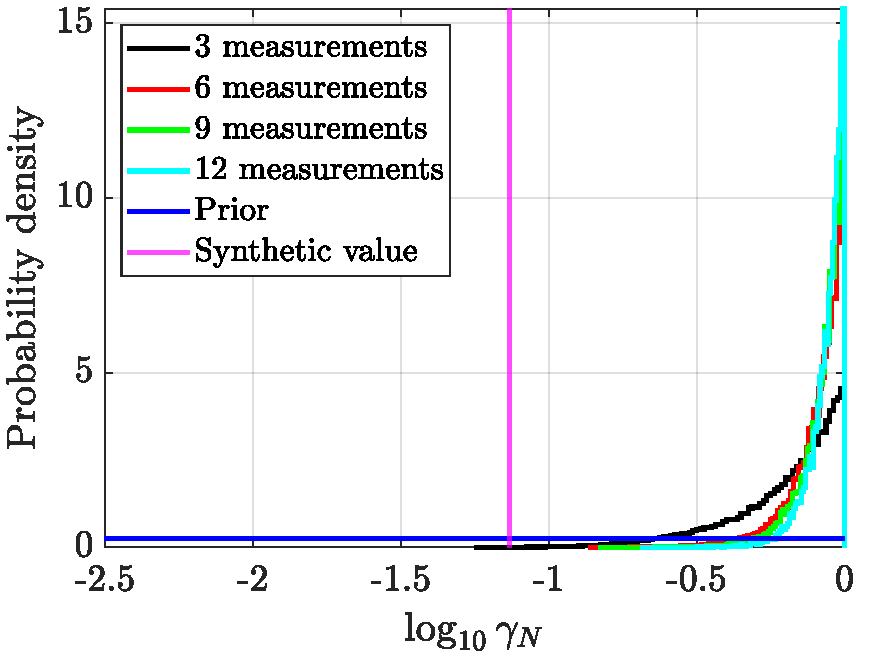
\includegraphics[width=\linewidth]{figures/cfd/Bayesian_gammaN_nme_bias.pdf}
      \caption{Posterior distribution of $\gamma_N$ without including a model error term in the likelihood function.}
      \label{fig:cfd:fig_gammaN_bias}
    \end{subfigure}
    \hfil
    \begin{subfigure}{0.47\linewidth}
      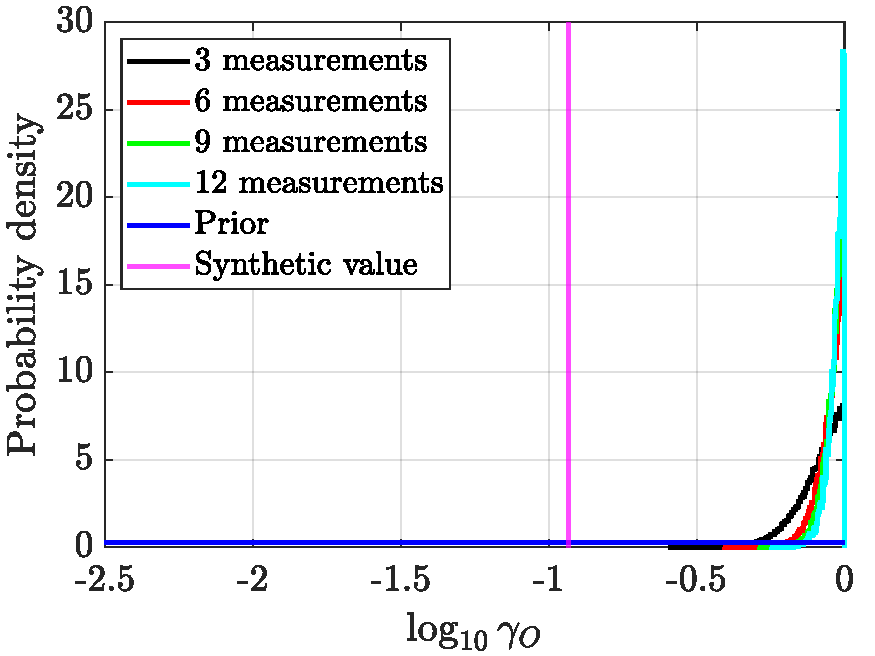
\includegraphics[width=\linewidth]{figures/cfd/Bayesian_gammaO_nme_bias.pdf}
      \caption{Posterior distribution of $\gamma_O$ without including a model error term in the likelihood function.}
      \label{fig:cfd:fig_gammaO_bias}
    \end{subfigure}
    \caption{Posterior distribution of $\gamma_N$ and $\gamma_O$ without including a model error term in the likelihood function. The vertical purple lines represent the true values of the catalytic coefficients.}
    \label{fig:cfd:fig_nme_bias}
\end{figure}

The results of the calibration without including a model error term in the likelihood function are shown in Fig.~\ref{fig:cfd:fig_nme_bias}, where the posterior distribution of $\gamma_N$ and $\gamma_O$ are reported. As we can see from Fig.~\ref{fig:cfd:fig_nme_bias}, we do not capture the true values of the catalytic coefficients (represented by the vertical purple lines) in the high probability region of the posterior distribution, as we increase the number of synthetic observations used for the calibration. The posterior mean concentrates around $\gamma_N, \gamma_O = 1.0$, which corresponds to a fully catalytic probe.

\smallskip
This behavior is expected, since the model sees a higher heat-flux than the one predicted by the surrogate model, and it tries to explain this discrepancy by increasing the catalytic coefficients. A practitioner can suspect the presence of a model error term by looking at the posterior-averaged distribution of the residuals. Calling $\mathbf{q}_w$ the vector of the observed heat-flux values, $\tilde{q}_{\mathrm{w}}(\mathbf{X}; \boldsymbol{\gamma})$ the vector of the surrogate predictions at the observed control variables $\mathbf{X} = \{(\mathrm{P}_0^{(i)}, \mathrm{P}_s^{(i)}, \dot{m}^{(i)})\}_{i=1}^{\nobs}$ and for a given value of the catalytic coefficients $\boldsymbol{\gamma} = \{\gamma_N, \gamma_O\}$, the calibration equation without a model error term can be written as,

\begin{equation}
    \mathbf{q}_w = \tilde{q}_{\mathrm{w}}(\mathbf{X}; \boldsymbol{\gamma}) + \boldsymbol{\epsilon} \;,
    \label{eq:cfd_cali_nme}
\end{equation}

where $\boldsymbol{\epsilon}$ is the vector of the measurement errors. Under Eq.~\eqref{eq:cfd_cali_nme}, the posterior-averaged residuals can be computed as,

\begin{equation}
    \mathbf{r} = \mathbb{E}_{\boldsymbol{\gamma} \sim \p{\boldsymbol{\gamma} \mid \data}} \left[ \mathbf{q}_w - \tilde{q}_{\mathrm{w}}(\mathbf{X}; \boldsymbol{\gamma})\right] = \boldsymbol{\epsilon} \;.
\end{equation}

Since we've made very strong assumptions on the measurement error term (zero mean and independent), we should see whether the residuals are consistent with these assumptions.

\begin{figure}[htbp]
  \centering
  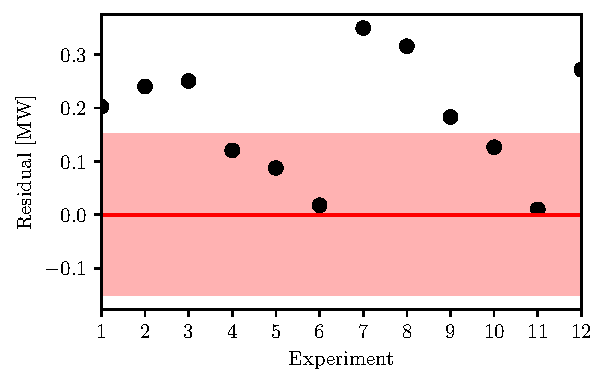
\includegraphics[width=0.5\textwidth]{figures/cfd/residuals_avg.pdf}
  \caption{Posterior-averaged residuals for the calibration without including a model error term in the likelihood function. The shaded region corresponds to the $95\%$ confidence interval of the measurement error term $\boldsymbol{\epsilon}$.}
  \label{fig:cfd:residuals_bias}
\end{figure}

Fig.~\ref{fig:cfd:residuals_bias} shows the posterior-averaged residuals for the calibration without including a model error term in the likelihood function. The shaded region corresponds to the $95\%$ confidence interval of the measurement error term $\boldsymbol{\epsilon}$. As we can see, many points fall outside the confidence interval, which is a strong indication that there is an additional source of discrepancy that is not captured by the measurement error term. Furthermore, all residuals are positive, which is a strong indication of the presence of an un-modeled bias in the calibration chain. 

\smallskip
In general, to convince a practitioner of the presence of a model error term, one needs many measurements to be able to look at the distribution of the residuals and check whether they are consistent with the assumptions made on the measurement error term. In this case, 12 measurements are sufficient to suspect the presence of a model error term, but in general, more measurements may be needed to be able to detect the presence of a model error term. A more robust way to detect the presence of a model error term is to actually perform a calibration with a model error term orthogonal to the model prediction (using Plumlee's orthogonality criterion, see \S\ref{sec:sota_1:identifiability}) and check whether the magnitude of $\mathbf{z}$ is significantly larger than the measurement error term $\boldsymbol{\epsilon}$. If this is the case, then we can be confident that there is a model error term in the calibration process. Note that forcing the model error term to be orthogonal to the model prediction may not be an ideal choice (especially in this case, where we are trying to infer a physical parameter) but a way to check whether there are un-modeled sources of discrepancies that can't be explained by the model.


\bigskip
To properly account for the presence of a bias term in the calibration process, we add a model error term $\mathbf{z} = z(\mathbf{X}; \bpsi)$ to Eq.~\eqref{eq:cfd_cali_nme}. We choose a model error term proportional to the true value of the heat flux, $z(.; \psi) = \psi \cdot \tilde{q}_{\mathrm{w}}(.; \boldsymbol{\gamma})$, where $\psi$ is a hyperparameter that we need to infer from the data (the proportionality constant of the bias term). In this case the model error term depends on $\boldsymbol{\gamma}$ and is \textbf{not} orthogonal to the model. We put a uniform prior on $\psi$ in the range $[-1, 1]$, which means that, before observing the data, we have no strong prior belief on the presence of a bias term in the calibration process. To estimate the posterior distribution of $\psi$, we can safely use the \gls{koh} method since, by physical intuition, we do not expect a correlation between $\psi$ and $\boldsymbol{\gamma}$.

\begin{equation}
  \psi_{\koh} = \argmax_{\psi \in [-1, 1]} \int_{\Gamma} \p{\data \mid \boldsymbol{\gamma}, \psi} \mathbb{P}(\dd \boldsymbol{\gamma}) \;.
  \label{eq:cfd:psikoh}
\end{equation}

To estimate the integral in Eq.~\eqref{eq:cfd:psikoh}, we can use a simple \gls{mc} method, which consists in sampling from the prior distribution of $\boldsymbol{\gamma}$ in $\Gamma = [-4,0] \times [-4,0]$. A non-gradient optimization method is used to find the optimal value of $\psi$ that maximizes the integral in Eq.~\eqref{eq:cfd:psikoh}. We use bootstrapping on the prior samples of $\boldsymbol{\gamma}$ to estimate the uncertainty on $\psi_{\koh}$.

\begin{table}[htbp]
\centering
\begin{tabular}{ccccc}
\hline
N. Measurements     & 3 & 6 & 9 & 12 \\ \hline
$\psi_{\koh}$ & $6.31\% \pm 0.035\%$ & $6.32\% \pm 0.022\%$ & $17.04\% \pm 0.039\%$ & $15.13\% \pm 0.33\%$ \\ 
\hline
\end{tabular}
\caption{\gls{koh} estimate of the bias term $\psi$ for different number of measurements used in the calibration process. The true value of $\psi$ is 0.15.}
\label{tab:cfd:KOHExpBias}
\end{table}

Tab.~\ref{tab:cfd:KOHExpBias} reports the \gls{koh} estimate of the bias term $\psi$ for different number of measurements used in the calibration process. The true value of $\psi$ is 0.15. The \gls{koh} method is able to correctly identify the presence of a bias term in the calibration process for all the different number of measurements used in the calibration process, and 12 measurements are needed to correctly estimate the true value of $\psi$ within the uncertainty. We now perform the Bayesian inversion to compute the posterior $\p{\boldsymbol{\gamma} \mid \data, \psi_{\koh}}$.

\begin{figure}[htbp]
    \centering
    \begin{subfigure}{0.47\linewidth}
      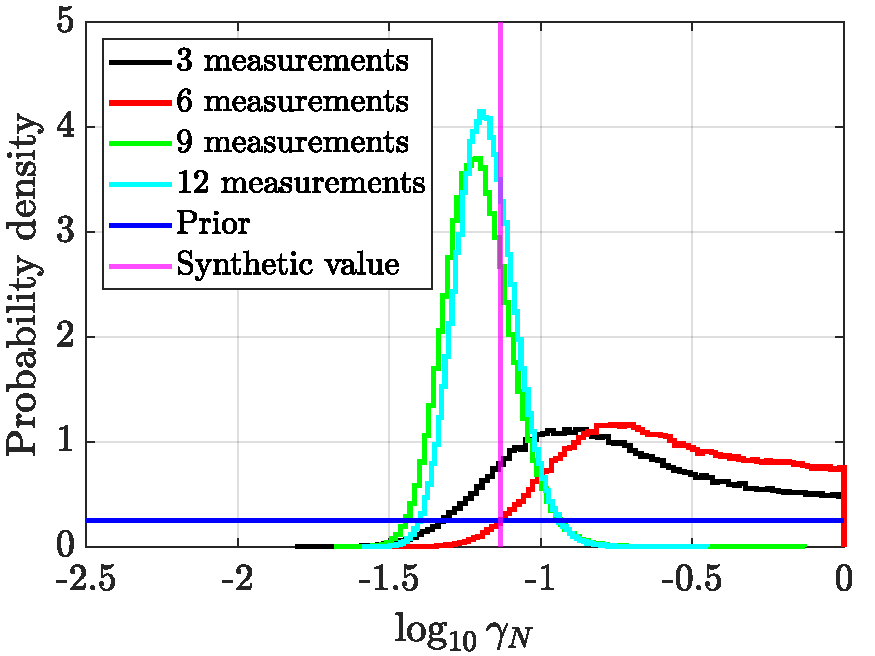
\includegraphics[width=\linewidth]{figures/cfd/Bayesian_gammaN_KOH_v2.pdf}
      \caption{Posterior distribution of $\gamma_N$.}
      \label{fig:cfd:fig_gammaN_koh}
    \end{subfigure}
    \hfil
    \begin{subfigure}{0.47\linewidth}
      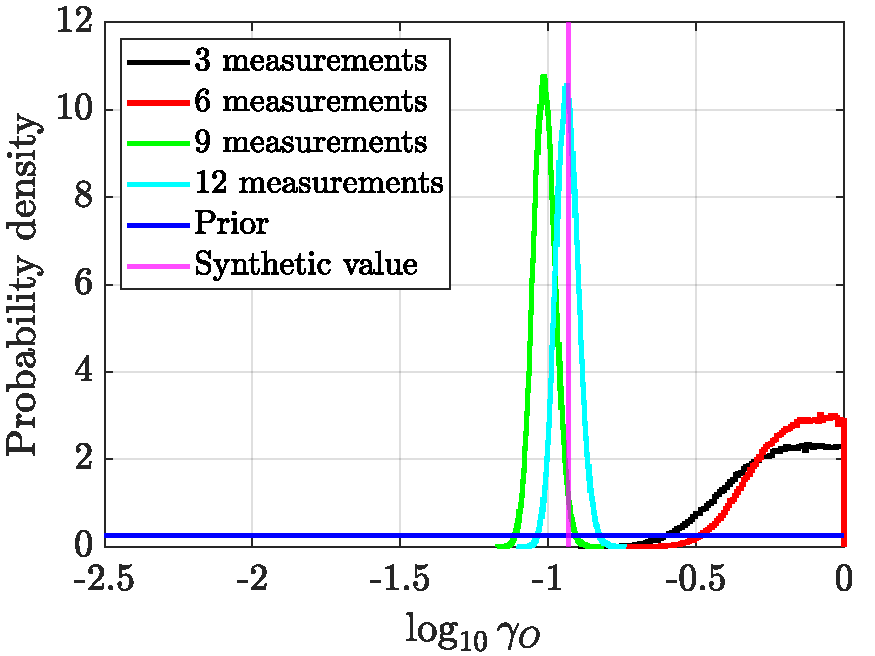
\includegraphics[width=\linewidth]{figures/cfd/Bayesian_gammaO_KOH_v2.pdf}
      \caption{Posterior distribution of $\gamma_O$. }
      \label{fig:cfd:fig_gammaO_koh}
    \end{subfigure}
    \caption{Marginal posterior distribution of $\gamma_N$ and $\gamma_O$ from $\p{\boldsymbol{\gamma} \mid \data, \psi_{\koh}}$. The vertical purple lines represent the true values of the catalytic coefficients.}
    \label{fig:cfd:fig_koh}
\end{figure}

The results of Fig.\ref{fig:cfd:fig_koh} shows that we can infer an excellent estimate of the true values of the catalytic coefficients $\gamma_N$ and $\gamma_O$ using approximately 9 measurements. Together with Tab.~\ref{tab:cfd:KOHExpBias}, these results show that the augmented calibration problem is well-posed and both the bias term and the catalytic coefficients are identifiable from the available measurements. This is a crucial result, since it means that we can indeed infer the true values of the catalytic coefficients from the available measurements even in the presence of a bias term, as long as we properly account for the presence of this bias term in the calibration process.


\subsubsection{Inadequate Model}
\label{sc:cfd:results:p1:inadequate}

We now consider the presence of a model discrepancy due to the use of an inadequate model. To do so, we use the \texttt{STAGLINE} surrogate model to calibrate against the synthetic data generated from the \gls{cfd} code. The calibration equation reads,

\begin{equation}
    \mathbf{q}_w = \tilde{q}_{\mathrm{w},\mathrm{stag}}(\mathbf{X}; \boldsymbol{\gamma}) + z(\mathbf{X}; \bpsi)+ \boldsymbol{\epsilon} \;.
\end{equation}

Before introducing the model error term $z(\mathbf{X}; \bpsi)$, we first perform the calibration of the surrogate model without including a model error term in the likelihood function and assume that the only discrepancy source is a random zero-mean Gaussian noise with a standard deviation proportional to $5\%$ of the observed value. 

\begin{figure}[htbp]
    \centering
    \begin{subfigure}{0.47\linewidth}
      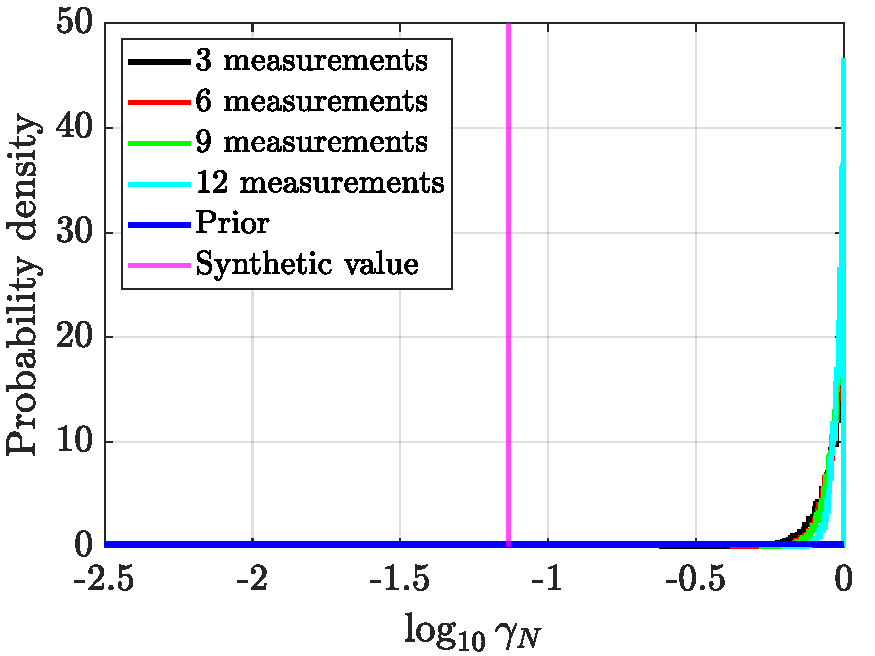
\includegraphics[width=\linewidth]{figures/cfd/Bayesian_gammaN_nme_stag.pdf}
      \caption{Posterior distribution of $\gamma_N$ without including a model error term in the likelihood function.}
      \label{fig:cfd:fig_gammaN_inadequate}
    \end{subfigure}
    \hfil
    \begin{subfigure}{0.47\linewidth}
      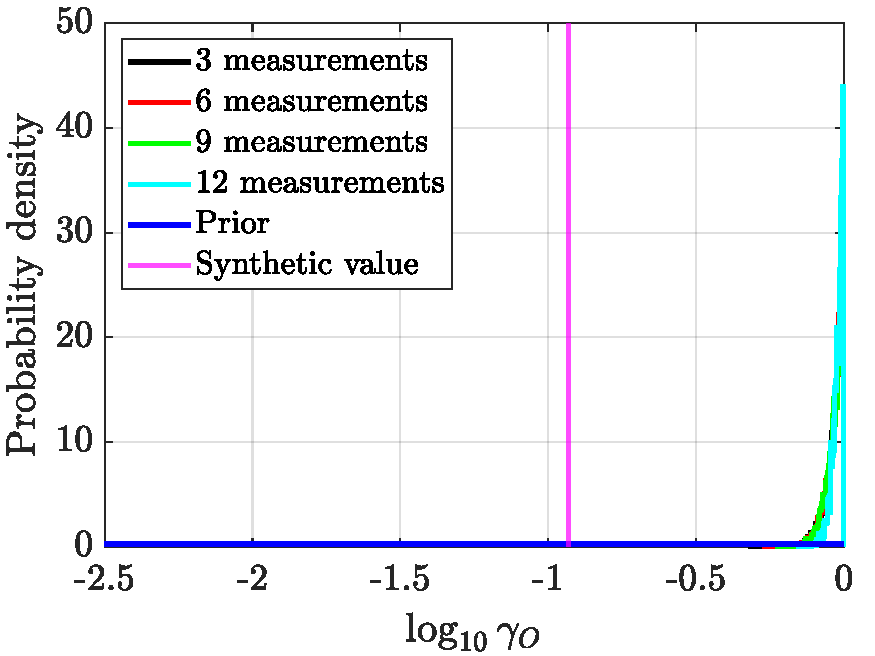
\includegraphics[width=\linewidth]{figures/cfd/Bayesian_gammaO_nme_stag.pdf}
      \caption{Posterior distribution of $\gamma_O$ without including a model error term in the likelihood function.}
      \label{fig:cfd:fig_gammaO_inadequate}
    \end{subfigure}
    \caption{Posterior distribution of $\gamma_N$ and $\gamma_O$ without including a model error term in the likelihood function. The vertical purple lines represent the true values of the catalytic coefficients.}
    \label{fig:cfd:fig_nme_inadequate}
\end{figure}

Similarly to the previous scenario, the results of the calibration without including a model error term in the likelihood function are shown in Fig.~\ref{fig:cfd:fig_nme_inadequate}, where the posterior distribution of $\gamma_N$ and $\gamma_O$ are reported. As we can see from Fig.~\ref{fig:cfd:fig_nme_inadequate}, we do not capture the true values of the catalytic coefficients (represented by the vertical purple lines) in the high probability region of the posterior distribution, as we increase the number of synthetic observations used for the calibration. The posterior mean concentrates around $\gamma_N, \gamma_O = 1.0$, which corresponds to a fully catalytic probe. 

\begin{figure}[htbp]
  \centering
  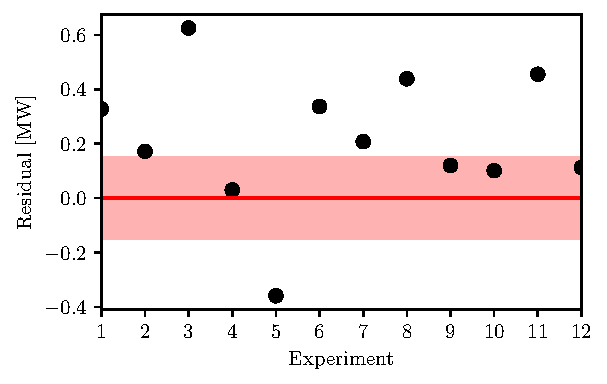
\includegraphics[width=0.5\textwidth]{figures/cfd/residuals_avg_stag.pdf}
  \caption{Posterior-averaged residuals for the calibration without including a model error term in the likelihood function. The shaded region corresponds to the $95\%$ confidence interval of the measurement error term $\boldsymbol{\epsilon}$.}
  \label{fig:cfd:residuals_inadequate}
\end{figure}

Fig.~\ref{fig:cfd:residuals_inadequate} confirms the presence of a model error by showing that many points fall outside the confidence interval of the measurement error term $\boldsymbol{\epsilon}$ and that the majority of the residuals are positive. The reason for the positive residuals is that the \texttt{STAGLINE} model is over-estimating the heat-flux values, and the calibration process tries to explain this discrepancy by increasing the catalytic coefficients.

\smallskip
Driven by the results of Fig.~\ref{fig:cfd:fig_nme_inadequate} and Fig.~\ref{fig:cfd:residuals_inadequate}, we introduce a model error term $z(\mathbf{p}; \bpsi)$ in the calibration process to account for the presence of a model discrepancy. For the model error term, we choose a constant mean \gls{gp} with an elliptic \gls{rbf} covariance, i.e. $z(.; \bpsi) \sim \mathcal{GP}(z; \mu, k_{\mathrm{RBF}}(.; \bpsi_{k}))$, where $\bpsi = (\mu, \sigma, \ell_{\mathrm{P}_0}, \ell_{\mathrm{P}_s}, \ell_{\dot{m}})$ are the hyperparameters of the model error term that we need to infer from the data.

\begin{table}[htbp]
\centering
\begin{tabular}{ccc}
\hline
Parameter                    & Min  & Max \\ \hline
$\sigma \ [\text{MW}/\text{m}^2]$  & 0 & 2  \\
$\ell_{\mathrm{P}_\text{0}} \ [\text{Pa}]$  & 10  & 19200  \\ 
$\ell_{\mathrm{P}_\text{s}} \ [\text{Pa}]$  & 1   & 300  \\ 
$\ell_{\dot{m}} \ [\text{g/s}]$     & 0.1 & 9  \\ \hline
\end{tabular}
\caption{Bounds on the non-informative uniform prior distribution.}
\label{tab:cfd:PriorModelErrorGP}
\end{table}

Tab.~\ref{tab:cfd:PriorModelErrorGP} reports the non-informative uniform prior distribution used for the hyperparameters of the model error term. 


\begin{figure}[htbp]
    \centering
    \begin{subfigure}{0.47\linewidth}
      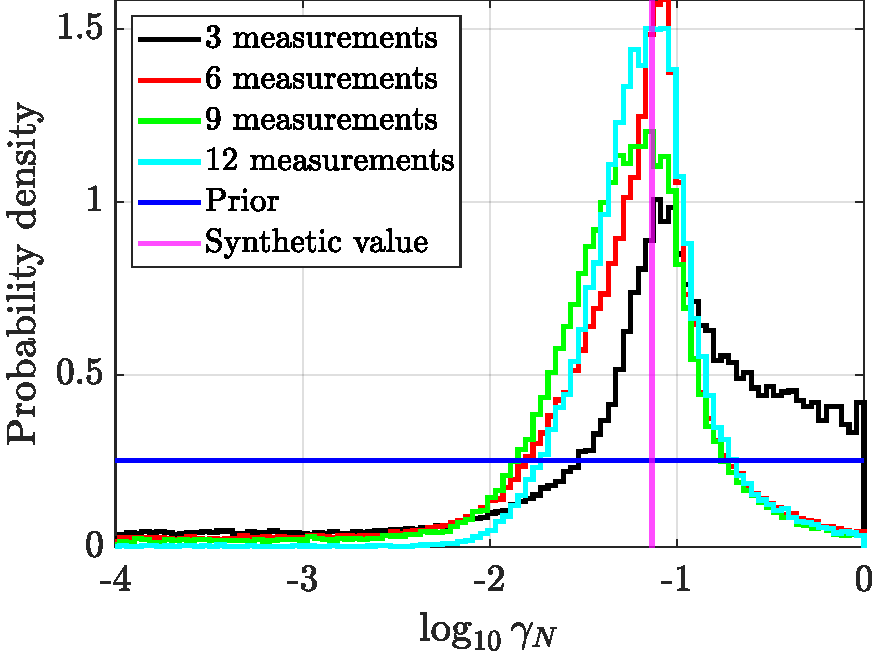
\includegraphics[width=\linewidth]{figures/cfd/Bayesian_gammaN_FullBayes.pdf}
      \caption{Posterior distribution of $\gamma_N$.}
      \label{fig:cfd:fig_gammaN_fullbayes}
    \end{subfigure}
    \hfil
    \begin{subfigure}{0.47\linewidth}
      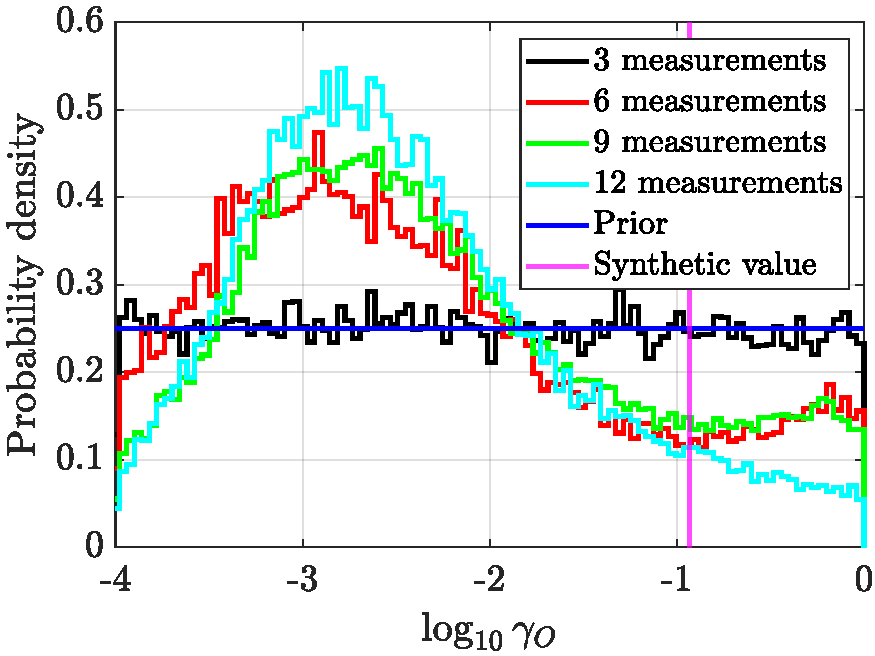
\includegraphics[width=\linewidth]{figures/cfd/Bayesian_gammaO_FullBayes.pdf}
      \caption{Posterior distribution of $\gamma_O$.}
      \label{fig:cfd:fig_gammaO_fullbayes}
    \end{subfigure}
    \caption{Posterior distribution of $\gamma_N$ and $\gamma_O$ with the \gls{fb} approach. The vertical purple lines represent the true values of the catalytic coefficients.}
    \label{fig:cfd:fig_fullbayes}
\end{figure}

\begin{table}[htbp]
\centering
\begin{tabular}{ccccc}
\hline
N. Measurements     & 3 & 6 & 9 & 12 \\ \hline
$\mu \ [\text{MW}/\text{m}^2]$ &  0.76  & 0.76 & 0.75 & 0.75 \\
$\sigma \ [\text{MW}/\text{m}^2]$  &  0.01  & 0.30  &  0.37 & 0.21 \\ 
$\ell_{\mathrm{P}_\text{0}} \ [\text{Pa}]$  &  17760 & 19104 & 19104 & 18727 \\
$\ell_{\dot{m}} \ [\text{g/s}]$    &  6.72 & 8.50 & 8.86 & 7.97 \\ 
\hline
\end{tabular}
\caption{\gls{map} value of the hyperparameters of the model error term for different number of measurements used in the calibration process.}
\label{tab:cfd:ModelErrorStag}
\end{table}

In Fig.~\ref{fig:cfd:fig_fullbayes} we show the results of the calibration with the \gls{fb} approach, where the model error term is included in the likelihood function and the hyperparameters of the model error term are marginalized out. We do not show the posterior distribution of the hyperparameters of the model error term, but we report in Tab.~\ref{tab:cfd:ModelErrorStag} the \gls{map} value of the hyperparameters of the model error term for different number of measurements used in the calibration process. The \gls{map} value is estimated from the \gls{mcmc} samples of the hyperparameters of the model error term by means of a kernel density estimation and a non-gradient optimization method. As we can see from Fig.~\ref{fig:cfd:fig_fullbayes}, we have an excellent estimate of the true values of the nitrogen catalytic coefficient $\gamma_N$ but a poor uncertainty reduction for the oxygen catalytic coefficient $\gamma_O$. 

\smallskip
We argue that the poor uncertainty reduction for $\gamma_O$ is due to the fact that our model is less sensitive to $\gamma_O$ than to $\gamma_N$, as evident in Fig.~\ref{fig:cfd:wellpose}. 


\begin{figure}
    \centering
    \begin{subfigure}{0.49\linewidth}
      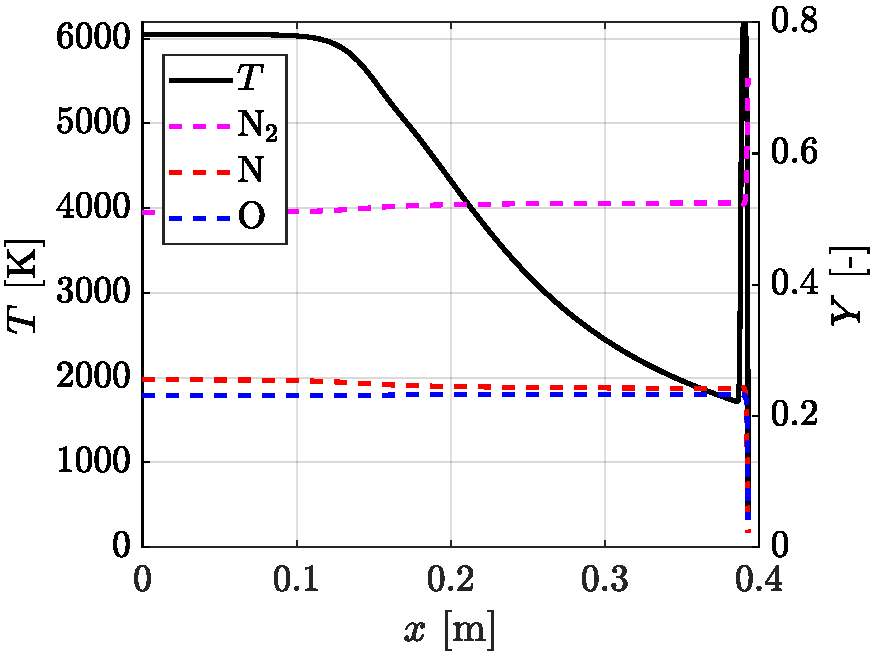
\includegraphics[width=\linewidth]{figures/cfd/Y.pdf}
      \caption{Entire domain.}
      \label{fig:cfd:Ydomain}
    \end{subfigure}
    \hfil
    \begin{subfigure}{0.49\linewidth}
      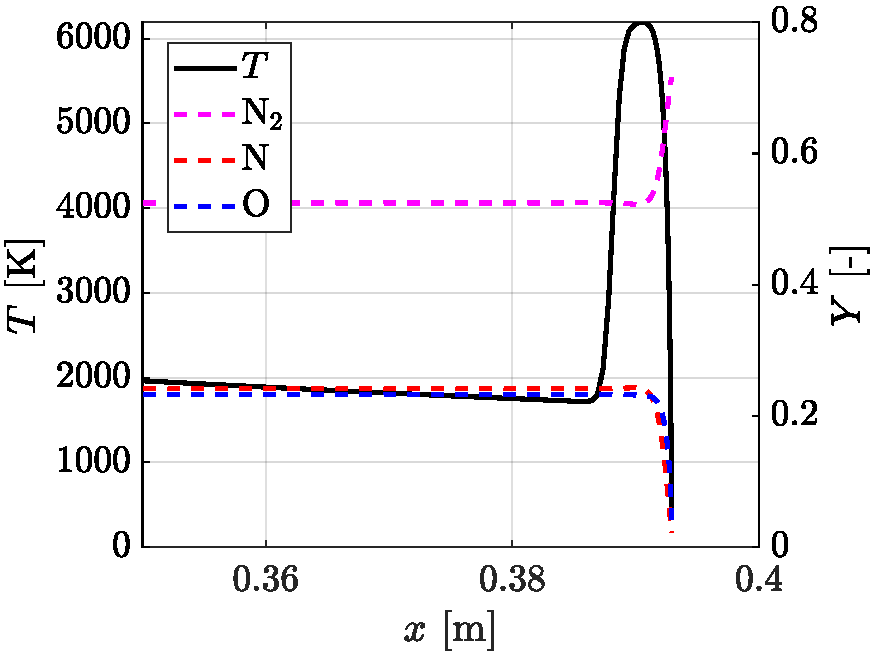
\includegraphics[width=\linewidth]{figures/cfd/Y_zoom.pdf}
      \caption{Zoomed-in view of Fig.~\ref{fig:cfd:Ydomain} near the probe.}
      \label{fig:cfd:Yzoom}
    \end{subfigure} 
    \caption{Mass fractions for $N_2$ $N$ and $O$ and temperature profiles along the centerline of the domain.}
    \label{fig:cfd:Y}
\end{figure}

In Fig.~\ref{fig:cfd:Y} we show the mass fractions for $N_2$ $N$ and $O$ and temperature profiles along the centerline of the domain. We can see that although nitrogen is not fully dissociated for the temperature range of this study (while oxygen is fully dissociated), the mass fraction of atomic nitrogen is similar to the mass fraction of atomic oxygen. The formation enthalpy of atomic nitrogen is higher than the formation enthalpy of atomic oxygen (472 kJ/mol vs 249 kJ/mol), which means that the heat-flux is more sensitive to changes in $\gamma_N$ than to changes in $\gamma_O$. This explains the poor uncertainty reduction for $\gamma_O$ in Fig.~\ref{fig:cfd:fig_fullbayes}.

\smallskip
In general, the results of this section show that estimating the true values of the catalytic coefficients from measurements of the heat-flux is a challenging problem, especially in the presence of a model error term. However, by properly accounting for the presence of a model error term in the calibration process, and properly designing the experiments, is possible to infer the true values of the catalytic coefficients from the available measurements, even in the presence of a model error term.


\subsection{Surrogate-based accelerated calibration}
\label{sec:cfd:results:p2}

In this section we present the results obtained with the \gls{as}-\gls{hgp} strategy for the calibration of the surrogate model of Eq.~\eqref{eq:cfd:mapping_surr}. As hinted in \S\ref{sc:cfd:methodology}, we artificially introduce a model error term by constructing the surrogate model of Eq.~\eqref{eq:cfd:mapping_surr} using only 10 \gls{cfd} simulations, which is not enough to capture the complexity of the \gls{cfd} model. We shall refer to the synthetic data generated with the \gls{cfd} code as the matrix $\mathbf{Y} = \{(q_{\mathrm{w}}^{(i)}, \mathrm{P}_{\mathrm{w}}^{(i)}, \dot{m}^{(i)})^{\top}\}_{i=1}^{\nobs}$, where $\nobs=14$ is the number of synthetic observations, and to the surrogate model of Eq.~\eqref{eq:cfd:mapping_surr} as $\tilde{\boldsymbol{f}}(\mathbf{X}; \boldsymbol{\theta})$, where $\boldsymbol{\theta} = (\mathrm{T}_0, \gamma_N)$ are the parameters that we want to calibrate and $\mathbf{X} = \{(\mathrm{P}_0^{(i)}, \mathrm{P}_s^{(i)})^{\top}\}_{i=1}^{\nobs}$ are the control variables of the experiments. Note that these values are reported in Tab.~\ref{tab:exp_data_2}. As stated in \S\ref{sc:cfd:methodology}, the model error term of each observable is then modeled as a zero-mean \gls{gp} with an elliptic \gls{rbf} covariance, i.e. $z_{i}(.; \bpsi) \sim \mathcal{GP}(z; 0, k_{\mathrm{RBF}}(.; \bpsi_{i}))$, where $\bpsi_i = (\sigma_{z_i}, \ell_{\mathrm{P}_0, z_i}, \ell_{\mathrm{P}_s, z_i})$ are the hyperparameters of the model error term that we need to infer from the data. We choose to use a non-informative uniform prior distribution for correlations lengths, $\ell_i$, and Jeffrey's prior for the kernel strengths, $\sigma_{z_i}$ \cite{uq_theory}. 

\smallskip
The results are obtained with the \gls{as}-\gls{hgp} strategy. For robustness, each test is repeated 30 times starting from different initial training sets and all the results (unless otherwise specified) are averaged over those repetitions.

\smallskip
We first analyze the computational cost of the iterative algorithm and the convergence of the error estimate, Eq.~\eqref{eq:fig_9b}, as a function of the training set size. Then, we compare the computational cost of a full \gls{mcmc} calibration using the exact \gls{cmp} method and the \gls{as}-\gls{hgp} strategy. Finally, we report the posterior density of the parameters obtained from the calibration process.

\begin{figure} [htbp]
    \begin{subfigure}{0.5\linewidth}
      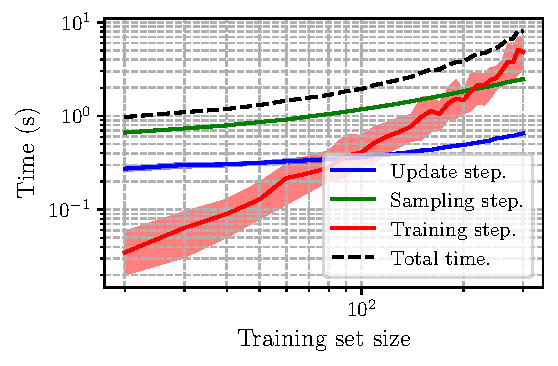
\includegraphics[width=\linewidth]{figures/surr/fig_9a.pdf}
      \caption{Computational time.}
      \label{fig:cfd:fig_9a}
    \end{subfigure}
    \hfil
    \begin{subfigure}{0.5\linewidth}
      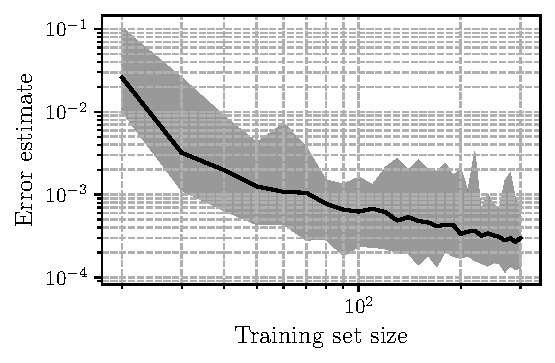
\includegraphics[width=\linewidth]{figures/surr/fig_9b.pdf}
      \caption{Convergence of the error estimate.}
      \label{fig:cfd:fig_9b}
    \end{subfigure}
    \caption{Computational time and convergence of the error estimate for the iterative algorithm. Shaded areas represent the $95\%$ confidence interval.}
    \label{fig:cfd:fig_9}
\end{figure}


In Fig.~\ref{fig:cfd:fig_9a} we show the time required to complete each step of the iterative algorithm as a function of the training set size. 
The dashed curve corresponds to the total computational time, which is the sum of the time required to train the surrogate model (i.e. estimate the hyperparameters of the hGPs see \S\ref{sc:surr:surrogate}), shown in red, the time required to sample the candidate set (see \S\ref{sc:surr:candidate}), shown in green, and the time required to update the training set (see \S\ref{sc:surr:select}), shown in blue.

\smallskip
In Fig.~\ref{fig:cfd:fig_9b} we show the convergence of the error estimate, Eq.~\eqref{eq:fig_9b}, as a function of the training set size. We can see that the error estimate, although converging, shows a high variability. The high variability is caused by the small size of the candidate set (here 200 points) which is used to estimate the expectation in Eq.~\eqref{eq:fig_9b}. As stated in \S\ref{sc:cfd:methodology}, this is not an issue since one could stop the iterative algorithm as soon as the error estimate is below a certain threshold for a certain number of iterations.

\begin{table}[htbp]
  \centering
  \begin{tabular}{|l|c|c|c|}
    \hline
    Method & Offline CPU time (s) & Online time ($\mu s$ per sample) & Total (s)\\
    \hline
    \gls{cmp} (exact) & 0 & 15150 $\pm$ 10 & $\approx 4.21$ h \\
    \hline
    \gls{as}-\gls{hgp} & 140 $\pm$ 10 & 120 $\pm$ 10 & $\approx 5$ min \\
    \hline
  \end{tabular}
    \caption{Computational cost comparison between \gls{cmp} and \gls{as}-\gls{hgp} strategies. The total time refers to a calibration with 1'000'000 \gls{mcmc} samples.}
    \label{tab:cfd:cost_comparison}
\end{table}

\smallskip
In Tab.~\ref{tab:cfd:cost_comparison} we report a comparison of the computational cost required to perform a full \gls{mcmc} calibration using the exact \gls{cmp} method and the \gls{as}-\gls{hgp} strategy of 1'000'000 samples. The speed-up obtained with the \gls{as}-\gls{hgp} strategy is considerable, reaching almost two orders of magnitude. Note that the speed-up depends on the total number of \gls{mcmc} samples used in the calibration process, since the offline cost of the \gls{as}-\gls{hgp} strategy is fixed while the online cost scales linearly with the number of \gls{mcmc} samples.


{
\captionsetup[figure]{skip=0ex} % <--- <---
\captionsetup[subfigure]{skip=0ex} % <--- <---
\begin{figure}[htbp]
\begin{subfigure}{0.5\linewidth}
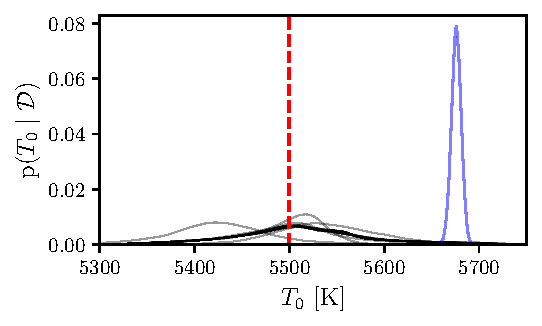
\includegraphics[width=\linewidth]{figures/surr/fig_10a.pdf}  % <---
  \caption{Reservoir temperature, $\mathrm{T}_0$.}
  \label{fig:10a}
\end{subfigure}
  \hfil
\begin{subfigure}{0.5\linewidth}
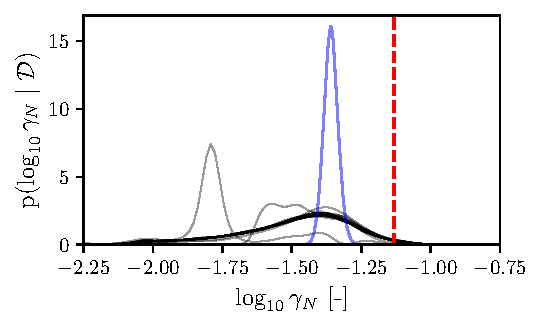
\includegraphics[width=\linewidth]{figures/surr/fig_10b.pdf} % <---
  \caption{Nitrogen catalytic coefficient, $\gamma_N$.}
  \label{fig:cfd:fig_10b}
\end{subfigure}
\begin{subfigure}{\linewidth}
  \centering
  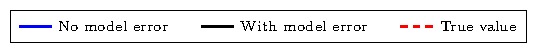
\includegraphics[width=0.7\linewidth]{figures/surr/fig_10c.pdf}
\end{subfigure}
\caption{Parameters' marginal distribution. Gradual color shading (from light to dark) illustrates the sequential progression of posterior distributions toward convergence.}
\label{fig:cfd:fig_10}
  \end{figure}
}

In Fig.~\ref{fig:cfd:fig_10} we report the \gls{kde} reconstruction of the posterior density of the parameters obtained from the calibration process. The different shading of the black curves indicates the effect of the number of training points on the posterior density. The \gls{hgp} posterior density indeed converges as the number of training points increases. The result of the calibration without the presence of the model error term is included, in blue, to stress the importance of including it since there is no value of the parameters that allows to match the experimental predictions. This can be seen in Fig.~\ref{fig:cfd:fig_10} as the calibration performs poorly with an overconfident and biased result. As far as the total temperature is concerned, including the model error term corrects the bias and the posterior distribution is centered around the true value. Interestingly, the posterior distribution is also less overconfident than the one obtained without the model error term, reflecting the uncertainty of the model itself. The same, however, cannot be said for the nitrogen catalytic coefficient, $\gamma_N$, which, although having a less overconfident marginal posterior, presents still a biased posterior. The bias is caused by the fact that the computer model is not precise enough in regions of the parameter space close to the true value, $\gamma_N \approx 0.09$ [-]. Indeed, Tab.~\ref{tab:training_data} shows that the training set does not properly cover that region of the parameter space and that more effort should be put in improving the model there.

\begin{figure}[htbp]
  \begin{subfigure}{0.5\linewidth}
    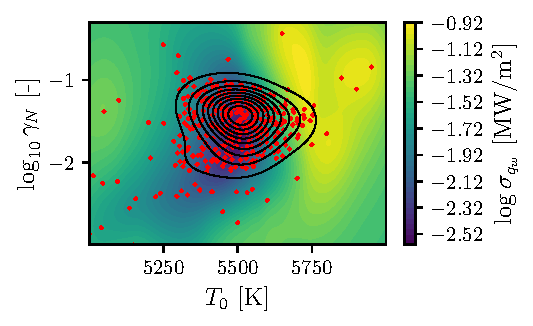
\includegraphics[width=\linewidth]{figures/surr/fig_11a.pdf}
    \caption{Heat flux, $q_{\mathrm{w}}$.}
  \end{subfigure}
  \hfil
  \begin{subfigure}{0.5\linewidth}
    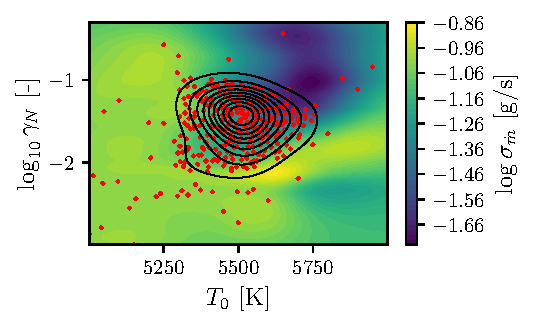
\includegraphics[width=\linewidth]{figures/surr/fig_11b.pdf}
    \caption{Mass flow rate, $\dot{m}$.}
  \end{subfigure}
    \caption{Predictive mean of the model error's covariance strength, $\sigma$, as function of the parameters. Black lines represent the posterior distribution while red dots the training set.}
    \label{fig:cfd:fig_11}
\end{figure}

In Fig.~\ref{fig:cfd:fig_11} we report the value of the predictive mean of the model error's covariance strength as a function of the parameters. The model error's covariance strength is reported just for the heat flux, $q_{\mathrm{w}}$, and mass flow rate, $\dot{m}$, since the one associated to the wall pressure, $\mathrm{P}_{\mathrm{w}}$, is smaller than the experimental error. In addition, we also show the \gls{kde} of the joint posterior distribution, $\p{\mathrm{T}_0, \log_{10} \gamma_N \mid \data}$ (black line), and the training set for the surrogate model (red dots) of the model error.
The model error for the heat flux is small when the temperature and the catalytic coefficient is small and increases as the temperature and the catalytic coefficient increase. The one associated to the mass flow rate has, instead, the opposite behavior.

\smallskip
The training set constructed with the iterative algorithm is able to capture the support of the posterior distribution and is more concentrated in the regions close to its mode. Nevertheless, we also observe some degree of dispersion as some points are also placed in regions where the posterior density is low. This is a desirable feature as we are not just interested in learning the posterior distribution but also the model error's behavior in the support.
Overall, the hGP approach is able to provide a cheap and good estimate of the posterior distribution of the parameters as well as a good estimate of the model error's behavior.


\begin{figure}[htbp]

\begin{subfigure}[t]{0.5\linewidth}
  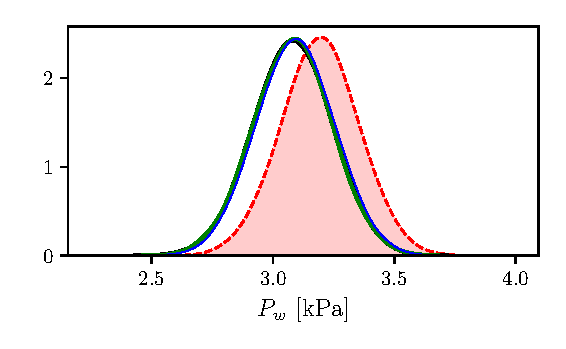
\includegraphics[width=\linewidth]{figures/surr/fig_12a.pdf}
  \caption{Wall pressure, $\mathrm{P}_{\mathrm{w}}$.}
\end{subfigure}
\hfil
\begin{subfigure}[t]{0.5\linewidth}
  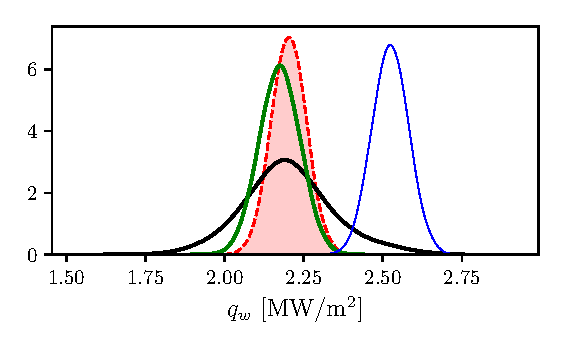
\includegraphics[width=\linewidth]{figures/surr/fig_12b.pdf}
  \caption{Heat flux, $q_{\mathrm{w}}$.}
\end{subfigure}

\medskip

\begin{subfigure}[t]{0.5\linewidth}
  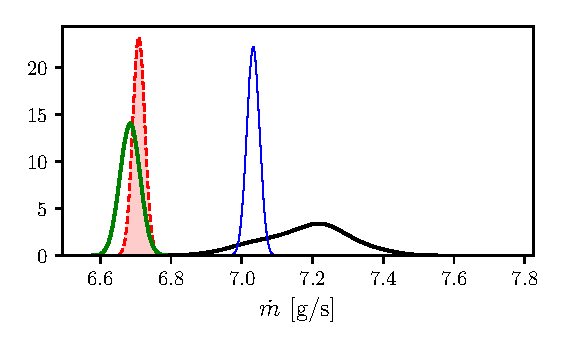
\includegraphics[width=\linewidth]{figures/surr/fig_12c.pdf}
  \caption{Mass flow rate, $\dot{m}$.}
\end{subfigure}
\hfil
\begin{subfigure}[t]{0.5\linewidth}
  \centering
  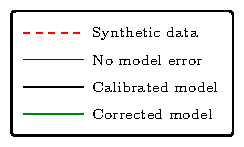
\includegraphics[width=0.7\linewidth]{figures/surr/fig_12d.pdf}
  \vspace{10pt}
\end{subfigure}

\caption{Posterior predictive distribution of an experiment of the 3 \glspl{qoi} at $P_0 = 14.14$ [kPa] and $P_s = 260.0$ [Pa].}
\label{fig:cfd:fig_12}
\end{figure}


Finally, we are also interested in assessing the predictive capabilities of the calibrated model and the effect of the model error correction. To do so, we evaluate the posterior predictive distribution not present in the training set, at $\bx = (\mathrm{P}_0, \mathrm{P}_s) = (14140, 260)\, \mathrm{[Pa]}$ with value $\mathbf{y} = (q_{\mathrm{w}}, \mathrm{P}_{\mathrm{w}}, \dot{m})$. We report three different predictions in Fig.~\ref{fig:cfd:fig_12} for each \gls{qoi}:
\begin{enumerate}

  \item The blue line corresponds to the prediction made without including the model error term. Here $\mathbf{y} = \hat{\mathbf{y}}(\bx; \btheta) + \boldsymbol{\epsilon}(\bx) \text{ with } \btheta \sim \p{\btheta \mid \data, \mathbf{z}=0}$. We do not include the model error term, and we use the posterior distribution of the parameters, $\btheta$, obtained from the calibration without the model error term.
  \item The black line corresponds to the prediction of the calibrated model. Here $\mathbf{y} = \hat{\mathbf{y}}(\bx; \btheta) + \boldsymbol{\epsilon}(\bx) \text{ with } \btheta \sim \tilde{\text{p}}(\btheta \mid \data)$. We do include the model error term but we use the posterior distribution of the parameters, $\btheta$, obtained from the hGP calibration, see Fig.~\ref{fig:cfd:fig_10}.
  \item The green line corresponds to the prediction of the corrected model. Here $\mathbf{y} = \hat{\mathbf{y}}(\bx; \btheta) + \mathbf{z}(\bx; \tilde{\bpsi}) + \boldsymbol{\epsilon}(\bx) \text{ with } \btheta \sim \tilde{\text{p}}(\btheta \mid \data)$. We do include the model error correction, and we use the posterior distribution of the parameters, $\btheta$, obtained from the hGP calibration, see Fig.~\ref{fig:cfd:fig_10}. The model error term is evaluated at the new point $\bx$ and the hyperparameters are sampled from the surrogate model.
\end{enumerate}

As we can see the prediction made without including the model error's term is biased and overconfident, except for the wall pressure, $\mathrm{P}_{\mathrm{w}}$, where the model error is small. Unsurprisingly, the prediction made with the calibrated model is less overconfident but still biased for the mass flow rate, $\dot{m}$. The bias is due to the presence of the model error term which, for the mass flow rate is large (see Fig.~\ref{fig:cfd:fig_11}). On the other hand, the prediction made with the corrected model is very close to the synthetic data. This means that we have been able to properly capture the model error's behavior and use it to correct the bias in the predictions. This is a crucial result since it shows that, even in the presence of a model error term, we can still make accurate predictions by properly accounting for the presence of this model error term in the calibration process.


\section{Conclusions}
\label{sc:cfd:conclusions}

In this chapter we have presented an interesting test case for the context of model calibration. The test case is based on the reconstruction of the catalytic coefficients of a probe used in high-enthalpy wind tunnel experiments. These catalytic coefficients are important parameters that affect the heat flux that a material experiences during a hypersonic flight, and their accurate estimation is crucial for the design of \glspl{tpm}. Since these coefficients pertain to a simplified description of the catalytic processes occurring on the probe's surface, they are not directly measurable and need to be inferred from measurements of a different quantity. This is where the model calibration process comes into play, as it allows us to reduce the uncertainty on the catalytic coefficients by comparing the predictions of a computer model with experimental measurements. 

\smallskip
After carefully reviewing the experimental setup available, we decided to use measurements of the heat flux, $q_{\mathrm{w}}$, as the quantity to calibrate against, since they are more sensitive to changes in the catalytic coefficients than measurements of other quantities, namely the wall pressure, $\mathrm{P}_{\mathrm{w}}$. In \S\ref{sc:cfd:numericalmodel} we described two numerical models that we use in this chapter: a complex \gls{cfd} code and a simplified solver and the corresponding surrogate models used to replace expensive queries to numerical solvers. 

\smallskip
In \S\ref{sc:cfd:methodology} we discussed the methodology used to obtain the results of this chapter. Since, at this stage no experimental data is available, we generate synthetic data from the \gls{cfd} code and we perform the calibration against this synthetic data. The results show that we can indeed infer the true values of the catalytic coefficients from the available measurements, even in the presence of a model error term, as long as we properly account for the presence of this model error term in the calibration process. We have shown how the presence of a model error term affects the calibration results and discussed how it can be detected. We have also shown how to properly account for two different sources of this model error term, namely a bias term and a model discrepancy due to the use of an inadequate model. Finally, we have also shown how the number of measurements used in the calibration process affects the results.

\smallskip
This chapter also marks the conclusion of the first part of this thesis, which was focused on the theoretical aspects of model calibration. In the previous two chapters we have introduced a novel adaptive surrogate-assisted calibration framework, which is able to provide a modular representation of the model error term and provide a good estimate of the posterior distribution of the parameters without needing to sample the model error term. For this reason, we have also shown an application of this framework to the test case of this chapter. We have shown that the \gls{cmp} method can indeed reduce the dimensionality of the problem and that the \gls{as}-\gls{hgp} strategy can provide a good estimate of the posterior distribution of the parameters with a considerable speed-up compared to a full \gls{mcmc} calibration using the exact \gls{cmp} method. We have also shown that the \gls{as}-\gls{hgp} strategy is able to provide a good estimate of the model error's behavior and use it to correct the bias in the predictions. 

\smallskip
Considerable work remains to be done in this scientific area. In particular, on a more experimental side, the next step would be to study other measurements that can be performed to better infer the catalytic coefficients. At this stage we have only used measurements of the heat flux, $q_{\mathrm{w}}$, but one could imagine using multiple probes at different locations or other sensors. Touching on a different aspect, one could investigate not only how many measurements are needed to properly infer the catalytic coefficients, but also how to optimally design the experiments to maximize the information gained from the measurements. This is an active area of research in the field of optimal experimental design, and we believe that applying optimal experimental design techniques, to the test case of this chapter would be an interesting research direction. Following a similar line of thought, one could also investigate the use of multi-fidelity surrogate models to further reduce the computational cost of the calibration process without sacrificing the accuracy of the results. Finally, once the experimental data will be available, it will be interesting to apply the methodologies discussed in this chapter to real data and compare the results with the ones obtained with synthetic data. This will allow us to validate the methodologies and to gain insights into the behavior of the catalytic coefficients in real conditions.